% Created by tikzDevice version 0.7.0 on 2014-06-30 20:14:20
% !TEX encoding = UTF-8 Unicode
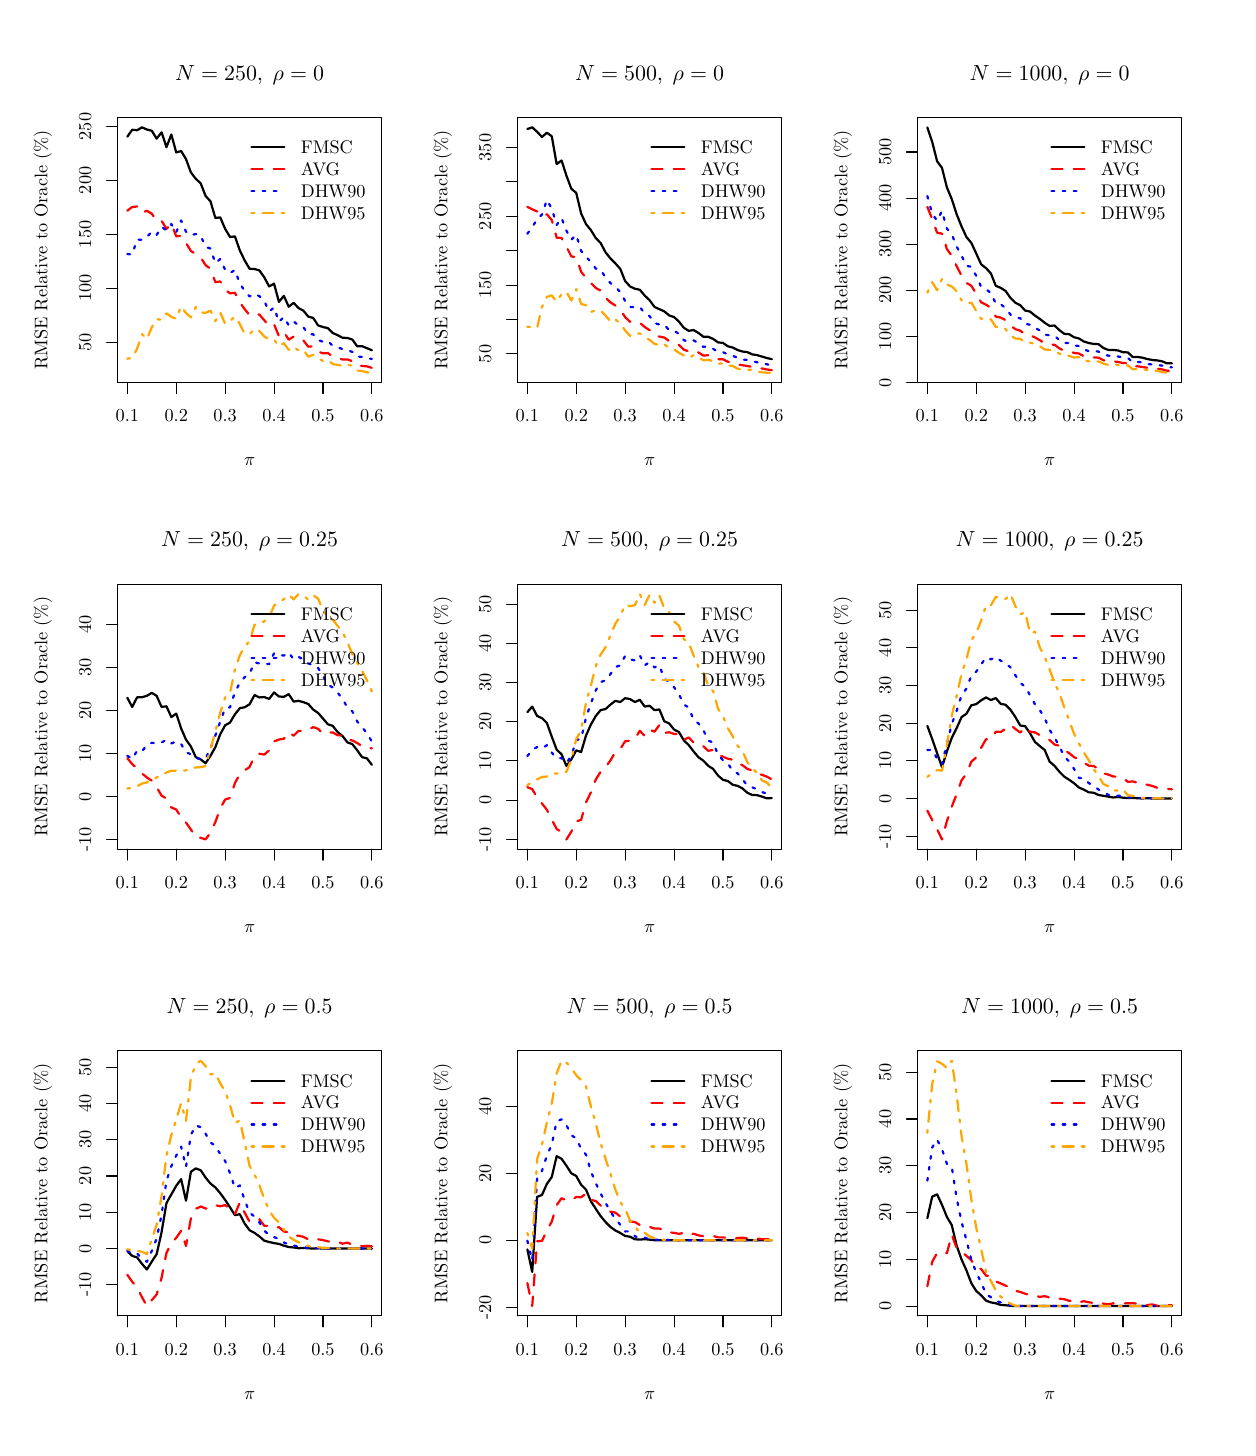
\begin{tikzpicture}[x=1pt,y=1pt]
\definecolor[named]{fillColor}{rgb}{1.00,1.00,1.00}
\path[use as bounding box,fill=fillColor,fill opacity=0.00] (0,0) rectangle (433.62,505.89);
\begin{scope}
\path[clip] ( 32.47,377.65) rectangle (127.91,473.42);
\definecolor[named]{drawColor}{rgb}{0.00,0.00,0.00}

\path[draw=drawColor,line width= 0.8pt,line join=round,line cap=round] ( 36.01,466.50) --
	( 37.77,468.99) --
	( 39.54,468.82) --
	( 41.31,469.87) --
	( 43.08,469.08) --
	( 44.84,468.64) --
	( 46.61,465.78) --
	( 48.38,468.06) --
	( 50.15,462.70) --
	( 51.91,467.27) --
	( 53.68,460.80) --
	( 55.45,461.32) --
	( 57.21,458.40) --
	( 58.98,453.57) --
	( 60.75,451.28) --
	( 62.52,449.63) --
	( 64.28,445.08) --
	( 66.05,443.15) --
	( 67.82,437.11) --
	( 69.59,437.33) --
	( 71.35,433.20) --
	( 73.12,430.23) --
	( 74.89,430.46) --
	( 76.66,425.40) --
	( 78.42,421.75) --
	( 80.19,418.76) --
	( 81.96,418.68) --
	( 83.72,418.17) --
	( 85.49,415.69) --
	( 87.26,412.38) --
	( 89.03,413.37) --
	( 90.79,406.80) --
	( 92.56,408.97) --
	( 94.33,405.06) --
	( 96.10,406.45) --
	( 97.86,404.57) --
	( 99.63,403.63) --
	(101.40,401.48) --
	(103.17,401.00) --
	(104.93,398.30) --
	(106.70,397.70) --
	(108.47,397.32) --
	(110.23,395.57) --
	(112.00,394.75) --
	(113.77,393.83) --
	(115.54,393.77) --
	(117.30,393.19) --
	(119.07,390.74) --
	(120.84,390.78) --
	(122.61,390.08) --
	(124.37,389.32);
\end{scope}
\begin{scope}
\path[clip] (  0.00,  0.00) rectangle (433.62,505.89);
\definecolor[named]{drawColor}{rgb}{0.00,0.00,0.00}

\path[draw=drawColor,line width= 0.4pt,line join=round,line cap=round] ( 36.01,377.65) -- (124.37,377.65);

\path[draw=drawColor,line width= 0.4pt,line join=round,line cap=round] ( 36.01,377.65) -- ( 36.01,373.69);

\path[draw=drawColor,line width= 0.4pt,line join=round,line cap=round] ( 53.68,377.65) -- ( 53.68,373.69);

\path[draw=drawColor,line width= 0.4pt,line join=round,line cap=round] ( 71.35,377.65) -- ( 71.35,373.69);

\path[draw=drawColor,line width= 0.4pt,line join=round,line cap=round] ( 89.03,377.65) -- ( 89.03,373.69);

\path[draw=drawColor,line width= 0.4pt,line join=round,line cap=round] (106.70,377.65) -- (106.70,373.69);

\path[draw=drawColor,line width= 0.4pt,line join=round,line cap=round] (124.37,377.65) -- (124.37,373.69);

\node[text=drawColor,anchor=base,inner sep=0pt, outer sep=0pt, scale=  0.66] at ( 36.01,363.40) {0.1};

\node[text=drawColor,anchor=base,inner sep=0pt, outer sep=0pt, scale=  0.66] at ( 53.68,363.40) {0.2};

\node[text=drawColor,anchor=base,inner sep=0pt, outer sep=0pt, scale=  0.66] at ( 71.35,363.40) {0.3};

\node[text=drawColor,anchor=base,inner sep=0pt, outer sep=0pt, scale=  0.66] at ( 89.03,363.40) {0.4};

\node[text=drawColor,anchor=base,inner sep=0pt, outer sep=0pt, scale=  0.66] at (106.70,363.40) {0.5};

\node[text=drawColor,anchor=base,inner sep=0pt, outer sep=0pt, scale=  0.66] at (124.37,363.40) {0.6};

\path[draw=drawColor,line width= 0.4pt,line join=round,line cap=round] ( 32.47,392.27) -- ( 32.47,470.18);

\path[draw=drawColor,line width= 0.4pt,line join=round,line cap=round] ( 32.47,392.27) -- ( 28.51,392.27);

\path[draw=drawColor,line width= 0.4pt,line join=round,line cap=round] ( 32.47,411.75) -- ( 28.51,411.75);

\path[draw=drawColor,line width= 0.4pt,line join=round,line cap=round] ( 32.47,431.22) -- ( 28.51,431.22);

\path[draw=drawColor,line width= 0.4pt,line join=round,line cap=round] ( 32.47,450.70) -- ( 28.51,450.70);

\path[draw=drawColor,line width= 0.4pt,line join=round,line cap=round] ( 32.47,470.18) -- ( 28.51,470.18);

\node[text=drawColor,rotate= 90.00,anchor=base,inner sep=0pt, outer sep=0pt, scale=  0.66] at ( 22.97,392.27) {50};

\node[text=drawColor,rotate= 90.00,anchor=base,inner sep=0pt, outer sep=0pt, scale=  0.66] at ( 22.97,411.75) {100};

\node[text=drawColor,rotate= 90.00,anchor=base,inner sep=0pt, outer sep=0pt, scale=  0.66] at ( 22.97,431.22) {150};

\node[text=drawColor,rotate= 90.00,anchor=base,inner sep=0pt, outer sep=0pt, scale=  0.66] at ( 22.97,450.70) {200};

\node[text=drawColor,rotate= 90.00,anchor=base,inner sep=0pt, outer sep=0pt, scale=  0.66] at ( 22.97,470.18) {250};

\path[draw=drawColor,line width= 0.4pt,line join=round,line cap=round] ( 32.47,377.65) --
	(127.91,377.65) --
	(127.91,473.42) --
	( 32.47,473.42) --
	( 32.47,377.65);
\end{scope}
\begin{scope}
\path[clip] (  0.00,337.26) rectangle (144.54,505.89);
\definecolor[named]{drawColor}{rgb}{0.00,0.00,0.00}

\node[text=drawColor,anchor=base,inner sep=0pt, outer sep=0pt, scale=  0.79] at ( 80.19,486.92) {\bfseries $N=250, \;\rho=0$};

\node[text=drawColor,anchor=base,inner sep=0pt, outer sep=0pt, scale=  0.66] at ( 80.19,347.56) {$\pi$};

\node[text=drawColor,rotate= 90.00,anchor=base,inner sep=0pt, outer sep=0pt, scale=  0.66] at (  7.13,425.53) {RMSE Relative to Oracle (\%)};
\end{scope}
\begin{scope}
\path[clip] ( 32.47,377.65) rectangle (127.91,473.42);
\definecolor[named]{drawColor}{rgb}{1.00,0.00,0.00}

\path[draw=drawColor,line width= 0.8pt,dash pattern=on 4pt off 4pt ,line join=round,line cap=round] ( 36.01,439.75) --
	( 37.77,441.08) --
	( 39.54,441.26) --
	( 41.31,438.95) --
	( 43.08,439.73) --
	( 44.84,438.67) --
	( 46.61,436.11) --
	( 48.38,436.12) --
	( 50.15,433.20) --
	( 51.91,435.03) --
	( 53.68,430.50) --
	( 55.45,430.65) --
	( 57.21,428.10) --
	( 58.98,425.19) --
	( 60.75,424.09) --
	( 62.52,422.87) --
	( 64.28,420.09) --
	( 66.05,418.71) --
	( 67.82,413.92) --
	( 69.59,414.19) --
	( 71.35,411.25) --
	( 73.12,409.87) --
	( 74.89,410.10) --
	( 76.66,406.66) --
	( 78.42,404.15) --
	( 80.19,402.03) --
	( 81.96,402.55) --
	( 83.72,402.21) --
	( 85.49,400.17) --
	( 87.26,397.99) --
	( 89.03,398.66) --
	( 90.79,394.43) --
	( 92.56,395.95) --
	( 94.33,393.14) --
	( 96.10,394.26) --
	( 97.86,393.05) --
	( 99.63,392.85) --
	(101.40,390.61) --
	(103.17,390.72) --
	(104.93,388.83) --
	(106.70,388.24) --
	(108.47,388.30) --
	(110.23,387.06) --
	(112.00,386.60) --
	(113.77,385.95) --
	(115.54,386.02) --
	(117.30,385.34) --
	(119.07,383.90) --
	(120.84,383.66) --
	(122.61,383.50) --
	(124.37,382.96);
\definecolor[named]{drawColor}{rgb}{0.00,0.00,1.00}

\path[draw=drawColor,line width= 0.8pt,dash pattern=on 1pt off 3pt ,line join=round,line cap=round] ( 36.01,424.09) --
	( 37.77,423.93) --
	( 39.54,429.35) --
	( 41.31,429.20) --
	( 43.08,430.23) --
	( 44.84,432.19) --
	( 46.61,431.03) --
	( 48.38,433.85) --
	( 50.15,432.69) --
	( 51.91,434.93) --
	( 53.68,431.95) --
	( 55.45,436.20) --
	( 57.21,432.17) --
	( 58.98,430.86) --
	( 60.75,431.32) --
	( 62.52,430.75) --
	( 64.28,426.63) --
	( 66.05,426.09) --
	( 67.82,420.75) --
	( 69.59,422.28) --
	( 71.35,418.38) --
	( 73.12,417.19) --
	( 74.89,418.35) --
	( 76.66,413.39) --
	( 78.42,410.81) --
	( 80.19,408.76) --
	( 81.96,409.68) --
	( 83.72,408.87) --
	( 85.49,407.10) --
	( 87.26,403.28) --
	( 89.03,404.82) --
	( 90.79,399.52) --
	( 92.56,401.38) --
	( 94.33,398.33) --
	( 96.10,399.79) --
	( 97.86,398.20) --
	( 99.63,397.63) --
	(101.40,395.14) --
	(103.17,395.09) --
	(104.93,393.03) --
	(106.70,392.37) --
	(108.47,392.61) --
	(110.23,390.94) --
	(112.00,390.32) --
	(113.77,389.76) --
	(115.54,389.41) --
	(117.30,388.71) --
	(119.07,387.04) --
	(120.84,386.90) --
	(122.61,386.52) --
	(124.37,386.17);
\definecolor[named]{drawColor}{rgb}{1.00,0.65,0.00}

\path[draw=drawColor,line width= 0.8pt,dash pattern=on 1pt off 3pt on 4pt off 3pt ,line join=round,line cap=round] ( 36.01,386.26) --
	( 37.77,386.55) --
	( 39.54,389.89) --
	( 41.31,395.15) --
	( 43.08,393.36) --
	( 44.84,397.60) --
	( 46.61,400.55) --
	( 48.38,400.34) --
	( 50.15,402.66) --
	( 51.91,401.39) --
	( 53.68,400.69) --
	( 55.45,405.20) --
	( 57.21,402.74) --
	( 58.98,401.21) --
	( 60.75,404.93) --
	( 62.52,403.02) --
	( 64.28,402.82) --
	( 66.05,403.64) --
	( 67.82,399.88) --
	( 69.59,402.98) --
	( 71.35,398.87) --
	( 73.12,399.89) --
	( 74.89,401.49) --
	( 76.66,398.81) --
	( 78.42,395.31) --
	( 80.19,395.15) --
	( 81.96,397.07) --
	( 83.72,396.22) --
	( 85.49,394.29) --
	( 87.26,393.28) --
	( 89.03,393.10) --
	( 90.79,390.73) --
	( 92.56,391.93) --
	( 94.33,389.46) --
	( 96.10,390.62) --
	( 97.86,389.21) --
	( 99.63,389.44) --
	(101.40,386.97) --
	(103.17,387.66) --
	(104.93,386.46) --
	(106.70,385.45) --
	(108.47,385.79) --
	(110.23,384.32) --
	(112.00,384.06) --
	(113.77,383.68) --
	(115.54,384.25) --
	(117.30,383.63) --
	(119.07,382.00) --
	(120.84,381.80) --
	(122.61,381.34) --
	(124.37,381.20);
\definecolor[named]{drawColor}{rgb}{0.00,0.00,0.00}

\path[draw=drawColor,line width= 0.8pt,line join=round,line cap=round] ( 80.89,462.63) -- ( 92.77,462.63);
\definecolor[named]{drawColor}{rgb}{1.00,0.00,0.00}

\path[draw=drawColor,line width= 0.8pt,dash pattern=on 4pt off 4pt ,line join=round,line cap=round] ( 80.89,454.71) -- ( 92.77,454.71);
\definecolor[named]{drawColor}{rgb}{0.00,0.00,1.00}

\path[draw=drawColor,line width= 0.8pt,dash pattern=on 1pt off 3pt ,line join=round,line cap=round] ( 80.89,446.79) -- ( 92.77,446.79);
\definecolor[named]{drawColor}{rgb}{1.00,0.65,0.00}

\path[draw=drawColor,line width= 0.8pt,dash pattern=on 1pt off 3pt on 4pt off 3pt ,line join=round,line cap=round] ( 80.89,438.87) -- ( 92.77,438.87);
\definecolor[named]{drawColor}{rgb}{0.00,0.00,0.00}

\node[text=drawColor,anchor=base west,inner sep=0pt, outer sep=0pt, scale=  0.66] at ( 98.71,460.35) {FMSC};

\node[text=drawColor,anchor=base west,inner sep=0pt, outer sep=0pt, scale=  0.66] at ( 98.71,452.43) {AVG};

\node[text=drawColor,anchor=base west,inner sep=0pt, outer sep=0pt, scale=  0.66] at ( 98.71,444.51) {DHW90};

\node[text=drawColor,anchor=base west,inner sep=0pt, outer sep=0pt, scale=  0.66] at ( 98.71,436.59) {DHW95};
\end{scope}
\begin{scope}
\path[clip] (177.01,377.65) rectangle (272.45,473.42);
\definecolor[named]{drawColor}{rgb}{0.00,0.00,0.00}

\path[draw=drawColor,line width= 0.8pt,line join=round,line cap=round] (180.55,469.26) --
	(182.31,469.87) --
	(184.08,468.27) --
	(185.85,466.38) --
	(187.62,467.93) --
	(189.38,466.64) --
	(191.15,456.59) --
	(192.92,457.89) --
	(194.69,452.39) --
	(196.45,447.68) --
	(198.22,446.19) --
	(199.99,438.74) --
	(201.75,434.90) --
	(203.52,432.73) --
	(205.29,429.86) --
	(207.06,428.05) --
	(208.82,424.69) --
	(210.59,422.49) --
	(212.36,420.71) --
	(214.13,418.72) --
	(215.89,414.33) --
	(217.66,412.37) --
	(219.43,411.55) --
	(221.20,411.18) --
	(222.96,409.08) --
	(224.73,407.39) --
	(226.50,404.97) --
	(228.26,404.17) --
	(230.03,403.37) --
	(231.80,401.90) --
	(233.57,401.31) --
	(235.33,399.68) --
	(237.10,397.44) --
	(238.87,396.33) --
	(240.64,396.62) --
	(242.40,395.57) --
	(244.17,394.18) --
	(245.94,394.18) --
	(247.71,393.41) --
	(249.47,392.16) --
	(251.24,391.97) --
	(253.01,390.75) --
	(254.77,390.31) --
	(256.54,389.39) --
	(258.31,388.86) --
	(260.08,388.63) --
	(261.84,387.82) --
	(263.61,387.56) --
	(265.38,387.02) --
	(267.15,386.50) --
	(268.91,386.10);
\end{scope}
\begin{scope}
\path[clip] (  0.00,  0.00) rectangle (433.62,505.89);
\definecolor[named]{drawColor}{rgb}{0.00,0.00,0.00}

\path[draw=drawColor,line width= 0.4pt,line join=round,line cap=round] (180.55,377.65) -- (268.91,377.65);

\path[draw=drawColor,line width= 0.4pt,line join=round,line cap=round] (180.55,377.65) -- (180.55,373.69);

\path[draw=drawColor,line width= 0.4pt,line join=round,line cap=round] (198.22,377.65) -- (198.22,373.69);

\path[draw=drawColor,line width= 0.4pt,line join=round,line cap=round] (215.89,377.65) -- (215.89,373.69);

\path[draw=drawColor,line width= 0.4pt,line join=round,line cap=round] (233.57,377.65) -- (233.57,373.69);

\path[draw=drawColor,line width= 0.4pt,line join=round,line cap=round] (251.24,377.65) -- (251.24,373.69);

\path[draw=drawColor,line width= 0.4pt,line join=round,line cap=round] (268.91,377.65) -- (268.91,373.69);

\node[text=drawColor,anchor=base,inner sep=0pt, outer sep=0pt, scale=  0.66] at (180.55,363.40) {0.1};

\node[text=drawColor,anchor=base,inner sep=0pt, outer sep=0pt, scale=  0.66] at (198.22,363.40) {0.2};

\node[text=drawColor,anchor=base,inner sep=0pt, outer sep=0pt, scale=  0.66] at (215.89,363.40) {0.3};

\node[text=drawColor,anchor=base,inner sep=0pt, outer sep=0pt, scale=  0.66] at (233.57,363.40) {0.4};

\node[text=drawColor,anchor=base,inner sep=0pt, outer sep=0pt, scale=  0.66] at (251.24,363.40) {0.5};

\node[text=drawColor,anchor=base,inner sep=0pt, outer sep=0pt, scale=  0.66] at (268.91,363.40) {0.6};

\path[draw=drawColor,line width= 0.4pt,line join=round,line cap=round] (177.01,388.00) -- (177.01,462.59);

\path[draw=drawColor,line width= 0.4pt,line join=round,line cap=round] (177.01,388.00) -- (173.05,388.00);

\path[draw=drawColor,line width= 0.4pt,line join=round,line cap=round] (177.01,400.43) -- (173.05,400.43);

\path[draw=drawColor,line width= 0.4pt,line join=round,line cap=round] (177.01,412.86) -- (173.05,412.86);

\path[draw=drawColor,line width= 0.4pt,line join=round,line cap=round] (177.01,425.29) -- (173.05,425.29);

\path[draw=drawColor,line width= 0.4pt,line join=round,line cap=round] (177.01,437.72) -- (173.05,437.72);

\path[draw=drawColor,line width= 0.4pt,line join=round,line cap=round] (177.01,450.15) -- (173.05,450.15);

\path[draw=drawColor,line width= 0.4pt,line join=round,line cap=round] (177.01,462.59) -- (173.05,462.59);

\node[text=drawColor,rotate= 90.00,anchor=base,inner sep=0pt, outer sep=0pt, scale=  0.66] at (167.51,388.00) {50};

\node[text=drawColor,rotate= 90.00,anchor=base,inner sep=0pt, outer sep=0pt, scale=  0.66] at (167.51,412.86) {150};

\node[text=drawColor,rotate= 90.00,anchor=base,inner sep=0pt, outer sep=0pt, scale=  0.66] at (167.51,437.72) {250};

\node[text=drawColor,rotate= 90.00,anchor=base,inner sep=0pt, outer sep=0pt, scale=  0.66] at (167.51,462.59) {350};

\path[draw=drawColor,line width= 0.4pt,line join=round,line cap=round] (177.01,377.65) --
	(272.45,377.65) --
	(272.45,473.42) --
	(177.01,473.42) --
	(177.01,377.65);
\end{scope}
\begin{scope}
\path[clip] (144.54,337.26) rectangle (289.08,505.89);
\definecolor[named]{drawColor}{rgb}{0.00,0.00,0.00}

\node[text=drawColor,anchor=base,inner sep=0pt, outer sep=0pt, scale=  0.79] at (224.73,486.92) {\bfseries $N=500, \;\rho=0$};

\node[text=drawColor,anchor=base,inner sep=0pt, outer sep=0pt, scale=  0.66] at (224.73,347.56) {$\pi$};

\node[text=drawColor,rotate= 90.00,anchor=base,inner sep=0pt, outer sep=0pt, scale=  0.66] at (151.67,425.53) {RMSE Relative to Oracle (\%)};
\end{scope}
\begin{scope}
\path[clip] (177.01,377.65) rectangle (272.45,473.42);
\definecolor[named]{drawColor}{rgb}{1.00,0.00,0.00}

\path[draw=drawColor,line width= 0.8pt,dash pattern=on 4pt off 4pt ,line join=round,line cap=round] (180.55,441.15) --
	(182.31,440.25) --
	(184.08,439.46) --
	(185.85,437.75) --
	(187.62,438.44) --
	(189.38,436.36) --
	(191.15,429.99) --
	(192.92,429.90) --
	(194.69,426.75) --
	(196.45,423.22) --
	(198.22,422.96) --
	(199.99,417.69) --
	(201.75,415.42) --
	(203.52,413.60) --
	(205.29,411.82) --
	(207.06,410.88) --
	(208.82,408.28) --
	(210.59,406.61) --
	(212.36,405.50) --
	(214.13,404.12) --
	(215.89,401.28) --
	(217.66,399.61) --
	(219.43,399.39) --
	(221.20,399.25) --
	(222.96,397.72) --
	(224.73,396.58) --
	(226.50,394.74) --
	(228.26,394.27) --
	(230.03,393.92) --
	(231.80,392.63) --
	(233.57,392.33) --
	(235.33,391.23) --
	(237.10,389.55) --
	(238.87,388.90) --
	(240.64,389.21) --
	(242.40,388.52) --
	(244.17,387.38) --
	(245.94,387.54) --
	(247.71,387.00) --
	(249.47,386.08) --
	(251.24,386.05) --
	(253.01,385.18) --
	(254.77,384.81) --
	(256.54,384.26) --
	(258.31,383.89) --
	(260.08,383.64) --
	(261.84,383.25) --
	(263.61,382.97) --
	(265.38,382.73) --
	(267.15,382.37) --
	(268.91,382.16);
\definecolor[named]{drawColor}{rgb}{0.00,0.00,1.00}

\path[draw=drawColor,line width= 0.8pt,dash pattern=on 1pt off 3pt ,line join=round,line cap=round] (180.55,431.40) --
	(182.31,433.79) --
	(184.08,436.64) --
	(185.85,438.38) --
	(187.62,443.64) --
	(189.38,440.50) --
	(191.15,434.60) --
	(192.92,437.13) --
	(194.69,432.50) --
	(196.45,429.26) --
	(198.22,431.04) --
	(199.99,425.19) --
	(201.75,423.11) --
	(203.52,421.22) --
	(205.29,418.82) --
	(207.06,418.44) --
	(208.82,415.55) --
	(210.59,413.60) --
	(212.36,412.20) --
	(214.13,410.34) --
	(215.89,407.14) --
	(217.66,405.01) --
	(219.43,404.83) --
	(221.20,404.91) --
	(222.96,402.71) --
	(224.73,401.65) --
	(226.50,399.10) --
	(228.26,398.66) --
	(230.03,398.47) --
	(231.80,396.61) --
	(233.57,396.41) --
	(235.33,395.24) --
	(237.10,392.97) --
	(238.87,392.31) --
	(240.64,392.89) --
	(242.40,391.90) --
	(244.17,390.54) --
	(245.94,390.64) --
	(247.71,389.81) --
	(249.47,388.69) --
	(251.24,388.63) --
	(253.01,387.83) --
	(254.77,387.32) --
	(256.54,386.58) --
	(258.31,385.95) --
	(260.08,385.83) --
	(261.84,385.39) --
	(263.61,384.94) --
	(265.38,384.72) --
	(267.15,384.25) --
	(268.91,383.77);
\definecolor[named]{drawColor}{rgb}{1.00,0.65,0.00}

\path[draw=drawColor,line width= 0.8pt,dash pattern=on 1pt off 3pt on 4pt off 3pt ,line join=round,line cap=round] (180.55,397.83) --
	(182.31,397.61) --
	(184.08,397.41) --
	(185.85,405.02) --
	(187.62,408.59) --
	(189.38,409.15) --
	(191.15,406.87) --
	(192.92,409.65) --
	(194.69,410.41) --
	(196.45,407.29) --
	(198.22,411.43) --
	(199.99,406.05) --
	(201.75,405.56) --
	(203.52,403.20) --
	(205.29,403.66) --
	(207.06,403.67) --
	(208.82,401.83) --
	(210.59,399.70) --
	(212.36,400.54) --
	(214.13,398.95) --
	(215.89,396.50) --
	(217.66,394.49) --
	(219.43,395.46) --
	(221.20,395.36) --
	(222.96,394.20) --
	(224.73,393.04) --
	(226.50,391.64) --
	(228.26,391.18) --
	(230.03,391.52) --
	(231.80,390.01) --
	(233.57,389.65) --
	(235.33,388.38) --
	(237.10,387.44) --
	(238.87,386.52) --
	(240.64,387.55) --
	(242.40,386.84) --
	(244.17,385.68) --
	(245.94,385.82) --
	(247.71,385.39) --
	(249.47,384.45) --
	(251.24,384.57) --
	(253.01,383.88) --
	(254.77,383.65) --
	(256.54,382.65) --
	(258.31,382.43) --
	(260.08,382.29) --
	(261.84,382.25) --
	(263.61,381.55) --
	(265.38,381.35) --
	(267.15,381.20) --
	(268.91,381.20);
\definecolor[named]{drawColor}{rgb}{0.00,0.00,0.00}

\path[draw=drawColor,line width= 0.8pt,line join=round,line cap=round] (225.43,462.63) -- (237.31,462.63);
\definecolor[named]{drawColor}{rgb}{1.00,0.00,0.00}

\path[draw=drawColor,line width= 0.8pt,dash pattern=on 4pt off 4pt ,line join=round,line cap=round] (225.43,454.71) -- (237.31,454.71);
\definecolor[named]{drawColor}{rgb}{0.00,0.00,1.00}

\path[draw=drawColor,line width= 0.8pt,dash pattern=on 1pt off 3pt ,line join=round,line cap=round] (225.43,446.79) -- (237.31,446.79);
\definecolor[named]{drawColor}{rgb}{1.00,0.65,0.00}

\path[draw=drawColor,line width= 0.8pt,dash pattern=on 1pt off 3pt on 4pt off 3pt ,line join=round,line cap=round] (225.43,438.87) -- (237.31,438.87);
\definecolor[named]{drawColor}{rgb}{0.00,0.00,0.00}

\node[text=drawColor,anchor=base west,inner sep=0pt, outer sep=0pt, scale=  0.66] at (243.25,460.35) {FMSC};

\node[text=drawColor,anchor=base west,inner sep=0pt, outer sep=0pt, scale=  0.66] at (243.25,452.43) {AVG};

\node[text=drawColor,anchor=base west,inner sep=0pt, outer sep=0pt, scale=  0.66] at (243.25,444.51) {DHW90};

\node[text=drawColor,anchor=base west,inner sep=0pt, outer sep=0pt, scale=  0.66] at (243.25,436.59) {DHW95};
\end{scope}
\begin{scope}
\path[clip] (321.55,377.65) rectangle (416.99,473.42);
\definecolor[named]{drawColor}{rgb}{0.00,0.00,0.00}

\path[draw=drawColor,line width= 0.8pt,line join=round,line cap=round] (325.09,469.87) --
	(326.85,464.60) --
	(328.62,457.60) --
	(330.39,455.22) --
	(332.16,448.15) --
	(333.92,443.94) --
	(335.69,438.44) --
	(337.46,434.05) --
	(339.23,430.21) --
	(340.99,428.11) --
	(342.76,424.28) --
	(344.53,420.37) --
	(346.29,419.00) --
	(348.06,417.07) --
	(349.83,412.59) --
	(351.60,411.87) --
	(353.36,410.75) --
	(355.13,408.24) --
	(356.90,406.48) --
	(358.67,405.60) --
	(360.43,403.66) --
	(362.20,403.30) --
	(363.97,401.85) --
	(365.74,400.64) --
	(367.50,399.26) --
	(369.27,398.10) --
	(371.04,398.26) --
	(372.80,396.60) --
	(374.57,395.26) --
	(376.34,395.11) --
	(378.11,394.02) --
	(379.87,393.58) --
	(381.64,392.48) --
	(383.41,391.94) --
	(385.18,391.61) --
	(386.94,391.52) --
	(388.71,390.14) --
	(390.48,389.42) --
	(392.25,389.45) --
	(394.01,389.24) --
	(395.78,388.61) --
	(397.55,388.54) --
	(399.31,386.88) --
	(401.08,386.89) --
	(402.85,386.63) --
	(404.62,386.13) --
	(406.38,385.81) --
	(408.15,385.65) --
	(409.92,385.32) --
	(411.69,384.60) --
	(413.45,384.60);
\end{scope}
\begin{scope}
\path[clip] (  0.00,  0.00) rectangle (433.62,505.89);
\definecolor[named]{drawColor}{rgb}{0.00,0.00,0.00}

\path[draw=drawColor,line width= 0.4pt,line join=round,line cap=round] (325.09,377.65) -- (413.45,377.65);

\path[draw=drawColor,line width= 0.4pt,line join=round,line cap=round] (325.09,377.65) -- (325.09,373.69);

\path[draw=drawColor,line width= 0.4pt,line join=round,line cap=round] (342.76,377.65) -- (342.76,373.69);

\path[draw=drawColor,line width= 0.4pt,line join=round,line cap=round] (360.43,377.65) -- (360.43,373.69);

\path[draw=drawColor,line width= 0.4pt,line join=round,line cap=round] (378.11,377.65) -- (378.11,373.69);

\path[draw=drawColor,line width= 0.4pt,line join=round,line cap=round] (395.78,377.65) -- (395.78,373.69);

\path[draw=drawColor,line width= 0.4pt,line join=round,line cap=round] (413.45,377.65) -- (413.45,373.69);

\node[text=drawColor,anchor=base,inner sep=0pt, outer sep=0pt, scale=  0.66] at (325.09,363.40) {0.1};

\node[text=drawColor,anchor=base,inner sep=0pt, outer sep=0pt, scale=  0.66] at (342.76,363.40) {0.2};

\node[text=drawColor,anchor=base,inner sep=0pt, outer sep=0pt, scale=  0.66] at (360.43,363.40) {0.3};

\node[text=drawColor,anchor=base,inner sep=0pt, outer sep=0pt, scale=  0.66] at (378.11,363.40) {0.4};

\node[text=drawColor,anchor=base,inner sep=0pt, outer sep=0pt, scale=  0.66] at (395.78,363.40) {0.5};

\node[text=drawColor,anchor=base,inner sep=0pt, outer sep=0pt, scale=  0.66] at (413.45,363.40) {0.6};

\path[draw=drawColor,line width= 0.4pt,line join=round,line cap=round] (321.55,377.68) -- (321.55,460.95);

\path[draw=drawColor,line width= 0.4pt,line join=round,line cap=round] (321.55,377.68) -- (317.59,377.68);

\path[draw=drawColor,line width= 0.4pt,line join=round,line cap=round] (321.55,394.34) -- (317.59,394.34);

\path[draw=drawColor,line width= 0.4pt,line join=round,line cap=round] (321.55,410.99) -- (317.59,410.99);

\path[draw=drawColor,line width= 0.4pt,line join=round,line cap=round] (321.55,427.64) -- (317.59,427.64);

\path[draw=drawColor,line width= 0.4pt,line join=round,line cap=round] (321.55,444.30) -- (317.59,444.30);

\path[draw=drawColor,line width= 0.4pt,line join=round,line cap=round] (321.55,460.95) -- (317.59,460.95);

\node[text=drawColor,rotate= 90.00,anchor=base,inner sep=0pt, outer sep=0pt, scale=  0.66] at (312.05,377.68) {0};

\node[text=drawColor,rotate= 90.00,anchor=base,inner sep=0pt, outer sep=0pt, scale=  0.66] at (312.05,394.34) {100};

\node[text=drawColor,rotate= 90.00,anchor=base,inner sep=0pt, outer sep=0pt, scale=  0.66] at (312.05,410.99) {200};

\node[text=drawColor,rotate= 90.00,anchor=base,inner sep=0pt, outer sep=0pt, scale=  0.66] at (312.05,427.64) {300};

\node[text=drawColor,rotate= 90.00,anchor=base,inner sep=0pt, outer sep=0pt, scale=  0.66] at (312.05,444.30) {400};

\node[text=drawColor,rotate= 90.00,anchor=base,inner sep=0pt, outer sep=0pt, scale=  0.66] at (312.05,460.95) {500};

\path[draw=drawColor,line width= 0.4pt,line join=round,line cap=round] (321.55,377.65) --
	(416.99,377.65) --
	(416.99,473.42) --
	(321.55,473.42) --
	(321.55,377.65);
\end{scope}
\begin{scope}
\path[clip] (289.08,337.26) rectangle (433.62,505.89);
\definecolor[named]{drawColor}{rgb}{0.00,0.00,0.00}

\node[text=drawColor,anchor=base,inner sep=0pt, outer sep=0pt, scale=  0.79] at (369.27,486.92) {\bfseries $N=1000, \;\rho=0$};

\node[text=drawColor,anchor=base,inner sep=0pt, outer sep=0pt, scale=  0.66] at (369.27,347.56) {$\pi$};

\node[text=drawColor,rotate= 90.00,anchor=base,inner sep=0pt, outer sep=0pt, scale=  0.66] at (296.21,425.53) {RMSE Relative to Oracle (\%)};
\end{scope}
\begin{scope}
\path[clip] (321.55,377.65) rectangle (416.99,473.42);
\definecolor[named]{drawColor}{rgb}{1.00,0.00,0.00}

\path[draw=drawColor,line width= 0.8pt,dash pattern=on 4pt off 4pt ,line join=round,line cap=round] (325.09,441.12) --
	(326.85,436.73) --
	(328.62,431.78) --
	(330.39,431.46) --
	(332.16,425.89) --
	(333.92,423.43) --
	(335.69,419.65) --
	(337.46,416.27) --
	(339.23,413.64) --
	(340.99,412.63) --
	(342.76,409.71) --
	(344.53,406.65) --
	(346.29,405.79) --
	(348.06,404.64) --
	(349.83,401.47) --
	(351.60,401.13) --
	(353.36,400.20) --
	(355.13,398.27) --
	(356.90,396.94) --
	(358.67,396.40) --
	(360.43,394.97) --
	(362.20,394.73) --
	(363.97,393.99) --
	(365.74,392.95) --
	(367.50,391.83) --
	(369.27,391.33) --
	(371.04,391.33) --
	(372.80,390.00) --
	(374.57,389.13) --
	(376.34,389.03) --
	(378.11,388.35) --
	(379.87,388.14) --
	(381.64,387.15) --
	(383.41,386.80) --
	(385.18,386.74) --
	(386.94,386.63) --
	(388.71,385.72) --
	(390.48,385.20) --
	(392.25,385.31) --
	(394.01,385.10) --
	(395.78,384.69) --
	(397.55,384.65) --
	(399.31,383.45) --
	(401.08,383.52) --
	(402.85,383.27) --
	(404.62,382.98) --
	(406.38,382.66) --
	(408.15,382.64) --
	(409.92,382.41) --
	(411.69,381.91) --
	(413.45,381.90);
\definecolor[named]{drawColor}{rgb}{0.00,0.00,1.00}

\path[draw=drawColor,line width= 0.8pt,dash pattern=on 1pt off 3pt ,line join=round,line cap=round] (325.09,445.06) --
	(326.85,438.61) --
	(328.62,436.14) --
	(330.39,439.65) --
	(332.16,433.28) --
	(333.92,431.24) --
	(335.69,426.73) --
	(337.46,423.51) --
	(339.23,419.85) --
	(340.99,419.45) --
	(342.76,416.21) --
	(344.53,412.24) --
	(346.29,411.39) --
	(348.06,410.00) --
	(349.83,406.15) --
	(351.60,405.94) --
	(353.36,404.56) --
	(355.13,402.20) --
	(356.90,401.15) --
	(358.67,400.88) --
	(360.43,398.89) --
	(362.20,398.53) --
	(363.97,397.39) --
	(365.74,396.48) --
	(367.50,394.94) --
	(369.27,394.74) --
	(371.04,394.60) --
	(372.80,392.97) --
	(374.57,391.94) --
	(376.34,391.97) --
	(378.11,391.03) --
	(379.87,390.86) --
	(381.64,389.57) --
	(383.41,389.03) --
	(385.18,389.11) --
	(386.94,388.83) --
	(388.71,387.76) --
	(390.48,387.39) --
	(392.25,387.08) --
	(394.01,387.07) --
	(395.78,386.69) --
	(397.55,386.57) --
	(399.31,384.92) --
	(401.08,385.12) --
	(402.85,384.94) --
	(404.62,384.33) --
	(406.38,384.18) --
	(408.15,384.05) --
	(409.92,383.76) --
	(411.69,383.17) --
	(413.45,383.15);
\definecolor[named]{drawColor}{rgb}{1.00,0.65,0.00}

\path[draw=drawColor,line width= 0.8pt,dash pattern=on 1pt off 3pt on 4pt off 3pt ,line join=round,line cap=round] (325.09,410.11) --
	(326.85,413.91) --
	(328.62,411.02) --
	(330.39,415.12) --
	(332.16,413.04) --
	(333.92,412.37) --
	(335.69,410.63) --
	(337.46,407.36) --
	(339.23,406.23) --
	(340.99,406.55) --
	(342.76,403.54) --
	(344.53,400.66) --
	(346.29,400.87) --
	(348.06,400.48) --
	(349.83,397.72) --
	(351.60,397.84) --
	(353.36,396.93) --
	(355.13,394.72) --
	(356.90,393.53) --
	(358.67,393.49) --
	(360.43,392.04) --
	(362.20,392.01) --
	(363.97,391.65) --
	(365.74,390.78) --
	(367.50,389.61) --
	(369.27,389.44) --
	(371.04,389.24) --
	(372.80,388.08) --
	(374.57,387.40) --
	(376.34,387.29) --
	(378.11,386.66) --
	(379.87,386.86) --
	(381.64,385.65) --
	(383.41,385.35) --
	(385.18,385.30) --
	(386.94,385.29) --
	(388.71,384.46) --
	(390.48,384.04) --
	(392.25,384.37) --
	(394.01,384.00) --
	(395.78,383.54) --
	(397.55,383.91) --
	(399.31,382.43) --
	(401.08,382.54) --
	(402.85,382.58) --
	(404.62,382.12) --
	(406.38,381.99) --
	(408.15,381.89) --
	(409.92,381.41) --
	(411.69,381.27) --
	(413.45,381.20);
\definecolor[named]{drawColor}{rgb}{0.00,0.00,0.00}

\path[draw=drawColor,line width= 0.8pt,line join=round,line cap=round] (369.97,462.63) -- (381.85,462.63);
\definecolor[named]{drawColor}{rgb}{1.00,0.00,0.00}

\path[draw=drawColor,line width= 0.8pt,dash pattern=on 4pt off 4pt ,line join=round,line cap=round] (369.97,454.71) -- (381.85,454.71);
\definecolor[named]{drawColor}{rgb}{0.00,0.00,1.00}

\path[draw=drawColor,line width= 0.8pt,dash pattern=on 1pt off 3pt ,line join=round,line cap=round] (369.97,446.79) -- (381.85,446.79);
\definecolor[named]{drawColor}{rgb}{1.00,0.65,0.00}

\path[draw=drawColor,line width= 0.8pt,dash pattern=on 1pt off 3pt on 4pt off 3pt ,line join=round,line cap=round] (369.97,438.87) -- (381.85,438.87);
\definecolor[named]{drawColor}{rgb}{0.00,0.00,0.00}

\node[text=drawColor,anchor=base west,inner sep=0pt, outer sep=0pt, scale=  0.66] at (387.79,460.35) {FMSC};

\node[text=drawColor,anchor=base west,inner sep=0pt, outer sep=0pt, scale=  0.66] at (387.79,452.43) {AVG};

\node[text=drawColor,anchor=base west,inner sep=0pt, outer sep=0pt, scale=  0.66] at (387.79,444.51) {DHW90};

\node[text=drawColor,anchor=base west,inner sep=0pt, outer sep=0pt, scale=  0.66] at (387.79,436.59) {DHW95};
\end{scope}
\begin{scope}
\path[clip] ( 32.47,209.02) rectangle (127.91,304.79);
\definecolor[named]{drawColor}{rgb}{0.00,0.00,0.00}

\path[draw=drawColor,line width= 0.8pt,line join=round,line cap=round] ( 36.01,263.75) --
	( 37.77,260.42) --
	( 39.54,263.91) --
	( 41.31,263.93) --
	( 43.08,264.47) --
	( 44.84,265.52) --
	( 46.61,264.44) --
	( 48.38,260.46) --
	( 50.15,260.66) --
	( 51.91,256.77) --
	( 53.68,258.02) --
	( 55.45,252.68) --
	( 57.21,248.62) --
	( 58.98,246.15) --
	( 60.75,242.29) --
	( 62.52,241.48) --
	( 64.28,240.07) --
	( 66.05,242.77) --
	( 67.82,245.90) --
	( 69.59,250.58) --
	( 71.35,253.79) --
	( 73.12,254.80) --
	( 74.89,257.77) --
	( 76.66,260.00) --
	( 78.42,260.32) --
	( 80.19,261.40) --
	( 81.96,264.73) --
	( 83.72,263.87) --
	( 85.49,264.00) --
	( 87.26,263.33) --
	( 89.03,265.66) --
	( 90.79,264.21) --
	( 92.56,264.08) --
	( 94.33,265.07) --
	( 96.10,262.36) --
	( 97.86,262.65) --
	( 99.63,262.16) --
	(101.40,261.49) --
	(103.17,259.47) --
	(104.93,258.28) --
	(106.70,256.25) --
	(108.47,254.18) --
	(110.23,253.59) --
	(112.00,251.36) --
	(113.77,249.93) --
	(115.54,247.62) --
	(117.30,247.01) --
	(119.07,244.78) --
	(120.84,242.29) --
	(122.61,241.84) --
	(124.37,239.53);
\end{scope}
\begin{scope}
\path[clip] (  0.00,  0.00) rectangle (433.62,505.89);
\definecolor[named]{drawColor}{rgb}{0.00,0.00,0.00}

\path[draw=drawColor,line width= 0.4pt,line join=round,line cap=round] ( 36.01,209.02) -- (124.37,209.02);

\path[draw=drawColor,line width= 0.4pt,line join=round,line cap=round] ( 36.01,209.02) -- ( 36.01,205.06);

\path[draw=drawColor,line width= 0.4pt,line join=round,line cap=round] ( 53.68,209.02) -- ( 53.68,205.06);

\path[draw=drawColor,line width= 0.4pt,line join=round,line cap=round] ( 71.35,209.02) -- ( 71.35,205.06);

\path[draw=drawColor,line width= 0.4pt,line join=round,line cap=round] ( 89.03,209.02) -- ( 89.03,205.06);

\path[draw=drawColor,line width= 0.4pt,line join=round,line cap=round] (106.70,209.02) -- (106.70,205.06);

\path[draw=drawColor,line width= 0.4pt,line join=round,line cap=round] (124.37,209.02) -- (124.37,205.06);

\node[text=drawColor,anchor=base,inner sep=0pt, outer sep=0pt, scale=  0.66] at ( 36.01,194.77) {0.1};

\node[text=drawColor,anchor=base,inner sep=0pt, outer sep=0pt, scale=  0.66] at ( 53.68,194.77) {0.2};

\node[text=drawColor,anchor=base,inner sep=0pt, outer sep=0pt, scale=  0.66] at ( 71.35,194.77) {0.3};

\node[text=drawColor,anchor=base,inner sep=0pt, outer sep=0pt, scale=  0.66] at ( 89.03,194.77) {0.4};

\node[text=drawColor,anchor=base,inner sep=0pt, outer sep=0pt, scale=  0.66] at (106.70,194.77) {0.5};

\node[text=drawColor,anchor=base,inner sep=0pt, outer sep=0pt, scale=  0.66] at (124.37,194.77) {0.6};

\path[draw=drawColor,line width= 0.4pt,line join=round,line cap=round] ( 32.47,212.52) -- ( 32.47,290.24);

\path[draw=drawColor,line width= 0.4pt,line join=round,line cap=round] ( 32.47,212.52) -- ( 28.51,212.52);

\path[draw=drawColor,line width= 0.4pt,line join=round,line cap=round] ( 32.47,228.06) -- ( 28.51,228.06);

\path[draw=drawColor,line width= 0.4pt,line join=round,line cap=round] ( 32.47,243.61) -- ( 28.51,243.61);

\path[draw=drawColor,line width= 0.4pt,line join=round,line cap=round] ( 32.47,259.15) -- ( 28.51,259.15);

\path[draw=drawColor,line width= 0.4pt,line join=round,line cap=round] ( 32.47,274.70) -- ( 28.51,274.70);

\path[draw=drawColor,line width= 0.4pt,line join=round,line cap=round] ( 32.47,290.24) -- ( 28.51,290.24);

\node[text=drawColor,rotate= 90.00,anchor=base,inner sep=0pt, outer sep=0pt, scale=  0.66] at ( 22.97,212.52) {-10};

\node[text=drawColor,rotate= 90.00,anchor=base,inner sep=0pt, outer sep=0pt, scale=  0.66] at ( 22.97,228.06) {0};

\node[text=drawColor,rotate= 90.00,anchor=base,inner sep=0pt, outer sep=0pt, scale=  0.66] at ( 22.97,243.61) {10};

\node[text=drawColor,rotate= 90.00,anchor=base,inner sep=0pt, outer sep=0pt, scale=  0.66] at ( 22.97,259.15) {20};

\node[text=drawColor,rotate= 90.00,anchor=base,inner sep=0pt, outer sep=0pt, scale=  0.66] at ( 22.97,274.70) {30};

\node[text=drawColor,rotate= 90.00,anchor=base,inner sep=0pt, outer sep=0pt, scale=  0.66] at ( 22.97,290.24) {40};

\path[draw=drawColor,line width= 0.4pt,line join=round,line cap=round] ( 32.47,209.02) --
	(127.91,209.02) --
	(127.91,304.79) --
	( 32.47,304.79) --
	( 32.47,209.02);
\end{scope}
\begin{scope}
\path[clip] (  0.00,168.63) rectangle (144.54,337.26);
\definecolor[named]{drawColor}{rgb}{0.00,0.00,0.00}

\node[text=drawColor,anchor=base,inner sep=0pt, outer sep=0pt, scale=  0.79] at ( 80.19,318.29) {\bfseries $N=250, \;\rho=0.25$};

\node[text=drawColor,anchor=base,inner sep=0pt, outer sep=0pt, scale=  0.66] at ( 80.19,178.93) {$\pi$};

\node[text=drawColor,rotate= 90.00,anchor=base,inner sep=0pt, outer sep=0pt, scale=  0.66] at (  7.13,256.90) {RMSE Relative to Oracle (\%)};
\end{scope}
\begin{scope}
\path[clip] ( 32.47,209.02) rectangle (127.91,304.79);
\definecolor[named]{drawColor}{rgb}{1.00,0.00,0.00}

\path[draw=drawColor,line width= 0.8pt,dash pattern=on 4pt off 4pt ,line join=round,line cap=round] ( 36.01,241.90) --
	( 37.77,239.77) --
	( 39.54,238.17) --
	( 41.31,236.40) --
	( 43.08,234.95) --
	( 44.84,233.78) --
	( 46.61,231.41) --
	( 48.38,228.41) --
	( 50.15,227.30) --
	( 51.91,224.11) --
	( 53.68,223.38) --
	( 55.45,220.48) --
	( 57.21,218.65) --
	( 58.98,216.15) --
	( 60.75,213.38) --
	( 62.52,213.13) --
	( 64.28,212.57) --
	( 66.05,215.00) --
	( 67.82,218.82) --
	( 69.59,223.83) --
	( 71.35,226.96) --
	( 73.12,227.56) --
	( 74.89,232.93) --
	( 76.66,236.18) --
	( 78.42,237.56) --
	( 80.19,238.70) --
	( 81.96,242.69) --
	( 83.72,243.51) --
	( 85.49,243.22) --
	( 87.26,244.76) --
	( 89.03,247.97) --
	( 90.79,248.66) --
	( 92.56,248.92) --
	( 94.33,251.31) --
	( 96.10,250.03) --
	( 97.86,251.78) --
	( 99.63,251.77) --
	(101.40,252.11) --
	(103.17,253.17) --
	(104.93,252.52) --
	(106.70,250.72) --
	(108.47,251.09) --
	(110.23,251.23) --
	(112.00,250.22) --
	(113.77,250.09) --
	(115.54,248.56) --
	(117.30,248.33) --
	(119.07,247.39) --
	(120.84,246.22) --
	(122.61,246.11) --
	(124.37,245.41);
\definecolor[named]{drawColor}{rgb}{0.00,0.00,1.00}

\path[draw=drawColor,line width= 0.8pt,dash pattern=on 1pt off 3pt ,line join=round,line cap=round] ( 36.01,242.79) --
	( 37.77,241.61) --
	( 39.54,244.62) --
	( 41.31,244.37) --
	( 43.08,246.71) --
	( 44.84,247.47) --
	( 46.61,247.36) --
	( 48.38,247.59) --
	( 50.15,248.58) --
	( 51.91,247.26) --
	( 53.68,247.92) --
	( 55.45,247.02) --
	( 57.21,244.05) --
	( 58.98,243.33) --
	( 60.75,241.93) --
	( 62.52,241.66) --
	( 64.28,241.74) --
	( 66.05,245.55) --
	( 67.82,250.12) --
	( 69.59,255.20) --
	( 71.35,259.95) --
	( 73.12,260.30) --
	( 74.89,265.80) --
	( 76.66,269.12) --
	( 78.42,271.23) --
	( 80.19,272.43) --
	( 81.96,276.59) --
	( 83.72,276.14) --
	( 85.49,276.06) --
	( 87.26,275.93) --
	( 89.03,279.83) --
	( 90.79,279.27) --
	( 92.56,278.98) --
	( 94.33,280.14) --
	( 96.10,277.61) --
	( 97.86,278.51) --
	( 99.63,277.61) --
	(101.40,276.14) --
	(103.17,275.52) --
	(104.93,274.54) --
	(106.70,271.73) --
	(108.47,268.48) --
	(110.23,267.47) --
	(112.00,265.62) --
	(113.77,263.32) --
	(115.54,260.19) --
	(117.30,258.85) --
	(119.07,255.19) --
	(120.84,253.06) --
	(122.61,250.98) --
	(124.37,247.90);
\definecolor[named]{drawColor}{rgb}{1.00,0.65,0.00}

\path[draw=drawColor,line width= 0.8pt,dash pattern=on 1pt off 3pt on 4pt off 3pt ,line join=round,line cap=round] ( 36.01,230.96) --
	( 37.77,231.18) --
	( 39.54,231.75) --
	( 41.31,232.75) --
	( 43.08,233.16) --
	( 44.84,234.47) --
	( 46.61,234.90) --
	( 48.38,236.07) --
	( 50.15,236.74) --
	( 51.91,237.42) --
	( 53.68,237.35) --
	( 55.45,237.37) --
	( 57.21,237.53) --
	( 58.98,238.37) --
	( 60.75,238.53) --
	( 62.52,238.69) --
	( 64.28,239.07) --
	( 66.05,245.29) --
	( 67.82,251.51) --
	( 69.59,258.37) --
	( 71.35,263.87) --
	( 73.12,265.51) --
	( 74.89,274.02) --
	( 76.66,279.08) --
	( 78.42,282.32) --
	( 80.19,284.18) --
	( 81.96,290.11) --
	( 83.72,290.37) --
	( 85.49,291.37) --
	( 87.26,292.85) --
	( 89.03,297.04) --
	( 90.79,298.35) --
	( 92.56,299.36) --
	( 94.33,301.05) --
	( 96.10,299.31) --
	( 97.86,301.24) --
	( 99.63,300.62) --
	(101.40,299.26) --
	(103.17,300.76) --
	(104.93,299.61) --
	(106.70,295.34) --
	(108.47,292.96) --
	(110.23,291.92) --
	(112.00,289.74) --
	(113.77,287.53) --
	(115.54,283.73) --
	(117.30,279.60) --
	(119.07,276.39) --
	(120.84,273.47) --
	(122.61,270.04) --
	(124.37,266.04);
\definecolor[named]{drawColor}{rgb}{0.00,0.00,0.00}

\path[draw=drawColor,line width= 0.8pt,line join=round,line cap=round] ( 80.89,294.00) -- ( 92.77,294.00);
\definecolor[named]{drawColor}{rgb}{1.00,0.00,0.00}

\path[draw=drawColor,line width= 0.8pt,dash pattern=on 4pt off 4pt ,line join=round,line cap=round] ( 80.89,286.08) -- ( 92.77,286.08);
\definecolor[named]{drawColor}{rgb}{0.00,0.00,1.00}

\path[draw=drawColor,line width= 0.8pt,dash pattern=on 1pt off 3pt ,line join=round,line cap=round] ( 80.89,278.16) -- ( 92.77,278.16);
\definecolor[named]{drawColor}{rgb}{1.00,0.65,0.00}

\path[draw=drawColor,line width= 0.8pt,dash pattern=on 1pt off 3pt on 4pt off 3pt ,line join=round,line cap=round] ( 80.89,270.24) -- ( 92.77,270.24);
\definecolor[named]{drawColor}{rgb}{0.00,0.00,0.00}

\node[text=drawColor,anchor=base west,inner sep=0pt, outer sep=0pt, scale=  0.66] at ( 98.71,291.72) {FMSC};

\node[text=drawColor,anchor=base west,inner sep=0pt, outer sep=0pt, scale=  0.66] at ( 98.71,283.80) {AVG};

\node[text=drawColor,anchor=base west,inner sep=0pt, outer sep=0pt, scale=  0.66] at ( 98.71,275.88) {DHW90};

\node[text=drawColor,anchor=base west,inner sep=0pt, outer sep=0pt, scale=  0.66] at ( 98.71,267.96) {DHW95};
\end{scope}
\begin{scope}
\path[clip] (177.01,209.02) rectangle (272.45,304.79);
\definecolor[named]{drawColor}{rgb}{0.00,0.00,0.00}

\path[draw=drawColor,line width= 0.8pt,line join=round,line cap=round] (180.55,258.53) --
	(182.31,260.56) --
	(184.08,257.18) --
	(185.85,256.37) --
	(187.62,254.61) --
	(189.38,249.70) --
	(191.15,245.00) --
	(192.92,243.32) --
	(194.69,239.08) --
	(196.45,241.48) --
	(198.22,244.76) --
	(199.99,244.12) --
	(201.75,250.10) --
	(203.52,254.08) --
	(205.29,257.17) --
	(207.06,259.30) --
	(208.82,259.67) --
	(210.59,261.27) --
	(212.36,262.64) --
	(214.13,262.20) --
	(215.89,263.60) --
	(217.66,263.27) --
	(219.43,262.21) --
	(221.20,263.00) --
	(222.96,260.57) --
	(224.73,260.86) --
	(226.50,259.28) --
	(228.26,259.53) --
	(230.03,255.27) --
	(231.80,254.46) --
	(233.57,252.27) --
	(235.33,251.34) --
	(237.10,248.37) --
	(238.87,246.64) --
	(240.64,244.34) --
	(242.40,242.26) --
	(244.17,240.99) --
	(245.94,239.15) --
	(247.71,238.00) --
	(249.47,235.64) --
	(251.24,234.11) --
	(253.01,233.65) --
	(254.77,232.32) --
	(256.54,231.92) --
	(258.31,230.97) --
	(260.08,229.38) --
	(261.84,228.64) --
	(263.61,228.55) --
	(265.38,228.01) --
	(267.15,227.39) --
	(268.91,227.52);
\end{scope}
\begin{scope}
\path[clip] (  0.00,  0.00) rectangle (433.62,505.89);
\definecolor[named]{drawColor}{rgb}{0.00,0.00,0.00}

\path[draw=drawColor,line width= 0.4pt,line join=round,line cap=round] (180.55,209.02) -- (268.91,209.02);

\path[draw=drawColor,line width= 0.4pt,line join=round,line cap=round] (180.55,209.02) -- (180.55,205.06);

\path[draw=drawColor,line width= 0.4pt,line join=round,line cap=round] (198.22,209.02) -- (198.22,205.06);

\path[draw=drawColor,line width= 0.4pt,line join=round,line cap=round] (215.89,209.02) -- (215.89,205.06);

\path[draw=drawColor,line width= 0.4pt,line join=round,line cap=round] (233.57,209.02) -- (233.57,205.06);

\path[draw=drawColor,line width= 0.4pt,line join=round,line cap=round] (251.24,209.02) -- (251.24,205.06);

\path[draw=drawColor,line width= 0.4pt,line join=round,line cap=round] (268.91,209.02) -- (268.91,205.06);

\node[text=drawColor,anchor=base,inner sep=0pt, outer sep=0pt, scale=  0.66] at (180.55,194.77) {0.1};

\node[text=drawColor,anchor=base,inner sep=0pt, outer sep=0pt, scale=  0.66] at (198.22,194.77) {0.2};

\node[text=drawColor,anchor=base,inner sep=0pt, outer sep=0pt, scale=  0.66] at (215.89,194.77) {0.3};

\node[text=drawColor,anchor=base,inner sep=0pt, outer sep=0pt, scale=  0.66] at (233.57,194.77) {0.4};

\node[text=drawColor,anchor=base,inner sep=0pt, outer sep=0pt, scale=  0.66] at (251.24,194.77) {0.5};

\node[text=drawColor,anchor=base,inner sep=0pt, outer sep=0pt, scale=  0.66] at (268.91,194.77) {0.6};

\path[draw=drawColor,line width= 0.4pt,line join=round,line cap=round] (177.01,212.63) -- (177.01,297.52);

\path[draw=drawColor,line width= 0.4pt,line join=round,line cap=round] (177.01,212.63) -- (173.05,212.63);

\path[draw=drawColor,line width= 0.4pt,line join=round,line cap=round] (177.01,226.78) -- (173.05,226.78);

\path[draw=drawColor,line width= 0.4pt,line join=round,line cap=round] (177.01,240.93) -- (173.05,240.93);

\path[draw=drawColor,line width= 0.4pt,line join=round,line cap=round] (177.01,255.08) -- (173.05,255.08);

\path[draw=drawColor,line width= 0.4pt,line join=round,line cap=round] (177.01,269.23) -- (173.05,269.23);

\path[draw=drawColor,line width= 0.4pt,line join=round,line cap=round] (177.01,283.37) -- (173.05,283.37);

\path[draw=drawColor,line width= 0.4pt,line join=round,line cap=round] (177.01,297.52) -- (173.05,297.52);

\node[text=drawColor,rotate= 90.00,anchor=base,inner sep=0pt, outer sep=0pt, scale=  0.66] at (167.51,212.63) {-10};

\node[text=drawColor,rotate= 90.00,anchor=base,inner sep=0pt, outer sep=0pt, scale=  0.66] at (167.51,226.78) {0};

\node[text=drawColor,rotate= 90.00,anchor=base,inner sep=0pt, outer sep=0pt, scale=  0.66] at (167.51,240.93) {10};

\node[text=drawColor,rotate= 90.00,anchor=base,inner sep=0pt, outer sep=0pt, scale=  0.66] at (167.51,255.08) {20};

\node[text=drawColor,rotate= 90.00,anchor=base,inner sep=0pt, outer sep=0pt, scale=  0.66] at (167.51,269.23) {30};

\node[text=drawColor,rotate= 90.00,anchor=base,inner sep=0pt, outer sep=0pt, scale=  0.66] at (167.51,283.37) {40};

\node[text=drawColor,rotate= 90.00,anchor=base,inner sep=0pt, outer sep=0pt, scale=  0.66] at (167.51,297.52) {50};

\path[draw=drawColor,line width= 0.4pt,line join=round,line cap=round] (177.01,209.02) --
	(272.45,209.02) --
	(272.45,304.79) --
	(177.01,304.79) --
	(177.01,209.02);
\end{scope}
\begin{scope}
\path[clip] (144.54,168.63) rectangle (289.08,337.26);
\definecolor[named]{drawColor}{rgb}{0.00,0.00,0.00}

\node[text=drawColor,anchor=base,inner sep=0pt, outer sep=0pt, scale=  0.79] at (224.73,318.29) {\bfseries $N=500, \;\rho=0.25$};

\node[text=drawColor,anchor=base,inner sep=0pt, outer sep=0pt, scale=  0.66] at (224.73,178.93) {$\pi$};

\node[text=drawColor,rotate= 90.00,anchor=base,inner sep=0pt, outer sep=0pt, scale=  0.66] at (151.67,256.90) {RMSE Relative to Oracle (\%)};
\end{scope}
\begin{scope}
\path[clip] (177.01,209.02) rectangle (272.45,304.79);
\definecolor[named]{drawColor}{rgb}{1.00,0.00,0.00}

\path[draw=drawColor,line width= 0.8pt,dash pattern=on 4pt off 4pt ,line join=round,line cap=round] (180.55,231.45) --
	(182.31,230.73) --
	(184.08,227.80) --
	(185.85,225.53) --
	(187.62,223.27) --
	(189.38,219.69) --
	(191.15,216.36) --
	(192.92,215.21) --
	(194.69,212.57) --
	(196.45,215.38) --
	(198.22,219.07) --
	(199.99,219.62) --
	(201.75,225.93) --
	(203.52,229.56) --
	(205.29,234.22) --
	(207.06,237.09) --
	(208.82,238.67) --
	(210.59,241.13) --
	(212.36,244.15) --
	(214.13,245.24) --
	(215.89,248.03) --
	(217.66,248.23) --
	(219.43,248.86) --
	(221.20,251.83) --
	(222.96,249.93) --
	(224.73,252.23) --
	(226.50,251.48) --
	(228.26,253.91) --
	(230.03,251.06) --
	(231.80,251.27) --
	(233.57,250.68) --
	(235.33,250.65) --
	(237.10,248.58) --
	(238.87,249.39) --
	(240.64,247.57) --
	(242.40,247.49) --
	(244.17,246.23) --
	(245.94,244.56) --
	(247.71,244.93) --
	(249.47,243.17) --
	(251.24,242.44) --
	(253.01,241.73) --
	(254.77,241.37) --
	(256.54,240.02) --
	(258.31,239.36) --
	(260.08,238.02) --
	(261.84,237.49) --
	(263.61,236.43) --
	(265.38,235.89) --
	(267.15,235.23) --
	(268.91,234.24);
\definecolor[named]{drawColor}{rgb}{0.00,0.00,1.00}

\path[draw=drawColor,line width= 0.8pt,dash pattern=on 1pt off 3pt ,line join=round,line cap=round] (180.55,242.67) --
	(182.31,244.84) --
	(184.08,245.97) --
	(185.85,245.42) --
	(187.62,246.61) --
	(189.38,243.92) --
	(191.15,241.90) --
	(192.92,241.95) --
	(194.69,240.20) --
	(196.45,242.72) --
	(198.22,248.43) --
	(199.99,248.97) --
	(201.75,256.55) --
	(203.52,261.75) --
	(205.29,266.43) --
	(207.06,269.39) --
	(208.82,270.08) --
	(210.59,272.30) --
	(212.36,274.83) --
	(214.13,275.47) --
	(215.89,278.90) --
	(217.66,277.66) --
	(219.43,277.24) --
	(221.20,279.07) --
	(222.96,275.47) --
	(224.73,276.65) --
	(226.50,274.71) --
	(228.26,275.42) --
	(230.03,270.61) --
	(231.80,269.54) --
	(233.57,267.54) --
	(235.33,265.05) --
	(237.10,261.28) --
	(238.87,260.24) --
	(240.64,255.73) --
	(242.40,254.46) --
	(244.17,252.05) --
	(245.94,248.24) --
	(247.71,247.59) --
	(249.47,243.07) --
	(251.24,241.23) --
	(253.01,240.04) --
	(254.77,237.28) --
	(256.54,236.43) --
	(258.31,234.24) --
	(260.08,232.02) --
	(261.84,231.38) --
	(263.61,230.63) --
	(265.38,229.67) --
	(267.15,229.09) --
	(268.91,228.45);
\definecolor[named]{drawColor}{rgb}{1.00,0.65,0.00}

\path[draw=drawColor,line width= 0.8pt,dash pattern=on 1pt off 3pt on 4pt off 3pt ,line join=round,line cap=round] (180.55,232.19) --
	(182.31,233.24) --
	(184.08,234.24) --
	(185.85,235.15) --
	(187.62,235.28) --
	(189.38,236.41) --
	(191.15,236.35) --
	(192.92,236.42) --
	(194.69,237.04) --
	(196.45,241.52) --
	(198.22,248.84) --
	(199.99,252.01) --
	(201.75,261.98) --
	(203.52,268.17) --
	(205.29,275.22) --
	(207.06,279.41) --
	(208.82,282.02) --
	(210.59,286.30) --
	(212.36,290.52) --
	(214.13,293.23) --
	(215.89,297.35) --
	(217.66,296.83) --
	(219.43,297.23) --
	(221.20,301.24) --
	(222.96,297.29) --
	(224.73,300.97) --
	(226.50,298.07) --
	(228.26,300.77) --
	(230.03,296.10) --
	(231.80,294.65) --
	(233.57,291.34) --
	(235.33,289.81) --
	(237.10,284.92) --
	(238.87,283.62) --
	(240.64,278.94) --
	(242.40,274.88) --
	(244.17,273.01) --
	(245.94,268.02) --
	(247.71,266.04) --
	(249.47,259.78) --
	(251.24,257.07) --
	(253.01,252.77) --
	(254.77,249.83) --
	(256.54,246.42) --
	(258.31,244.50) --
	(260.08,240.42) --
	(261.84,238.27) --
	(263.61,236.45) --
	(265.38,233.85) --
	(267.15,233.07) --
	(268.91,231.17);
\definecolor[named]{drawColor}{rgb}{0.00,0.00,0.00}

\path[draw=drawColor,line width= 0.8pt,line join=round,line cap=round] (225.43,294.00) -- (237.31,294.00);
\definecolor[named]{drawColor}{rgb}{1.00,0.00,0.00}

\path[draw=drawColor,line width= 0.8pt,dash pattern=on 4pt off 4pt ,line join=round,line cap=round] (225.43,286.08) -- (237.31,286.08);
\definecolor[named]{drawColor}{rgb}{0.00,0.00,1.00}

\path[draw=drawColor,line width= 0.8pt,dash pattern=on 1pt off 3pt ,line join=round,line cap=round] (225.43,278.16) -- (237.31,278.16);
\definecolor[named]{drawColor}{rgb}{1.00,0.65,0.00}

\path[draw=drawColor,line width= 0.8pt,dash pattern=on 1pt off 3pt on 4pt off 3pt ,line join=round,line cap=round] (225.43,270.24) -- (237.31,270.24);
\definecolor[named]{drawColor}{rgb}{0.00,0.00,0.00}

\node[text=drawColor,anchor=base west,inner sep=0pt, outer sep=0pt, scale=  0.66] at (243.25,291.72) {FMSC};

\node[text=drawColor,anchor=base west,inner sep=0pt, outer sep=0pt, scale=  0.66] at (243.25,283.80) {AVG};

\node[text=drawColor,anchor=base west,inner sep=0pt, outer sep=0pt, scale=  0.66] at (243.25,275.88) {DHW90};

\node[text=drawColor,anchor=base west,inner sep=0pt, outer sep=0pt, scale=  0.66] at (243.25,267.96) {DHW95};
\end{scope}
\begin{scope}
\path[clip] (321.55,209.02) rectangle (416.99,304.79);
\definecolor[named]{drawColor}{rgb}{0.00,0.00,0.00}

\path[draw=drawColor,line width= 0.8pt,line join=round,line cap=round] (325.09,253.61) --
	(326.85,248.81) --
	(328.62,243.72) --
	(330.39,238.65) --
	(332.16,244.38) --
	(333.92,249.25) --
	(335.69,252.78) --
	(337.46,256.77) --
	(339.23,258.00) --
	(340.99,261.04) --
	(342.76,261.44) --
	(344.53,262.82) --
	(346.29,263.87) --
	(348.06,262.91) --
	(349.83,263.64) --
	(351.60,261.55) --
	(353.36,261.22) --
	(355.13,259.42) --
	(356.90,256.79) --
	(358.67,253.71) --
	(360.43,253.48) --
	(362.20,250.92) --
	(363.97,247.79) --
	(365.74,246.29) --
	(367.50,244.87) --
	(369.27,240.68) --
	(371.04,239.16) --
	(372.80,237.02) --
	(374.57,235.23) --
	(376.34,234.13) --
	(378.11,232.86) --
	(379.87,231.32) --
	(381.64,230.54) --
	(383.41,229.59) --
	(385.18,229.43) --
	(386.94,228.62) --
	(388.71,228.33) --
	(390.48,228.02) --
	(392.25,227.72) --
	(394.01,227.89) --
	(395.78,227.64) --
	(397.55,227.53) --
	(399.31,227.57) --
	(401.08,227.44) --
	(402.85,227.37) --
	(404.62,227.43) --
	(406.38,227.37) --
	(408.15,227.37) --
	(409.92,227.37) --
	(411.69,227.37) --
	(413.45,227.37);
\end{scope}
\begin{scope}
\path[clip] (  0.00,  0.00) rectangle (433.62,505.89);
\definecolor[named]{drawColor}{rgb}{0.00,0.00,0.00}

\path[draw=drawColor,line width= 0.4pt,line join=round,line cap=round] (325.09,209.02) -- (413.45,209.02);

\path[draw=drawColor,line width= 0.4pt,line join=round,line cap=round] (325.09,209.02) -- (325.09,205.06);

\path[draw=drawColor,line width= 0.4pt,line join=round,line cap=round] (342.76,209.02) -- (342.76,205.06);

\path[draw=drawColor,line width= 0.4pt,line join=round,line cap=round] (360.43,209.02) -- (360.43,205.06);

\path[draw=drawColor,line width= 0.4pt,line join=round,line cap=round] (378.11,209.02) -- (378.11,205.06);

\path[draw=drawColor,line width= 0.4pt,line join=round,line cap=round] (395.78,209.02) -- (395.78,205.06);

\path[draw=drawColor,line width= 0.4pt,line join=round,line cap=round] (413.45,209.02) -- (413.45,205.06);

\node[text=drawColor,anchor=base,inner sep=0pt, outer sep=0pt, scale=  0.66] at (325.09,194.77) {0.1};

\node[text=drawColor,anchor=base,inner sep=0pt, outer sep=0pt, scale=  0.66] at (342.76,194.77) {0.2};

\node[text=drawColor,anchor=base,inner sep=0pt, outer sep=0pt, scale=  0.66] at (360.43,194.77) {0.3};

\node[text=drawColor,anchor=base,inner sep=0pt, outer sep=0pt, scale=  0.66] at (378.11,194.77) {0.4};

\node[text=drawColor,anchor=base,inner sep=0pt, outer sep=0pt, scale=  0.66] at (395.78,194.77) {0.5};

\node[text=drawColor,anchor=base,inner sep=0pt, outer sep=0pt, scale=  0.66] at (413.45,194.77) {0.6};

\path[draw=drawColor,line width= 0.4pt,line join=round,line cap=round] (321.55,213.77) -- (321.55,295.37);

\path[draw=drawColor,line width= 0.4pt,line join=round,line cap=round] (321.55,213.77) -- (317.59,213.77);

\path[draw=drawColor,line width= 0.4pt,line join=round,line cap=round] (321.55,227.37) -- (317.59,227.37);

\path[draw=drawColor,line width= 0.4pt,line join=round,line cap=round] (321.55,240.97) -- (317.59,240.97);

\path[draw=drawColor,line width= 0.4pt,line join=round,line cap=round] (321.55,254.57) -- (317.59,254.57);

\path[draw=drawColor,line width= 0.4pt,line join=round,line cap=round] (321.55,268.17) -- (317.59,268.17);

\path[draw=drawColor,line width= 0.4pt,line join=round,line cap=round] (321.55,281.77) -- (317.59,281.77);

\path[draw=drawColor,line width= 0.4pt,line join=round,line cap=round] (321.55,295.37) -- (317.59,295.37);

\node[text=drawColor,rotate= 90.00,anchor=base,inner sep=0pt, outer sep=0pt, scale=  0.66] at (312.05,213.77) {-10};

\node[text=drawColor,rotate= 90.00,anchor=base,inner sep=0pt, outer sep=0pt, scale=  0.66] at (312.05,227.37) {0};

\node[text=drawColor,rotate= 90.00,anchor=base,inner sep=0pt, outer sep=0pt, scale=  0.66] at (312.05,240.97) {10};

\node[text=drawColor,rotate= 90.00,anchor=base,inner sep=0pt, outer sep=0pt, scale=  0.66] at (312.05,254.57) {20};

\node[text=drawColor,rotate= 90.00,anchor=base,inner sep=0pt, outer sep=0pt, scale=  0.66] at (312.05,268.17) {30};

\node[text=drawColor,rotate= 90.00,anchor=base,inner sep=0pt, outer sep=0pt, scale=  0.66] at (312.05,281.77) {40};

\node[text=drawColor,rotate= 90.00,anchor=base,inner sep=0pt, outer sep=0pt, scale=  0.66] at (312.05,295.37) {50};

\path[draw=drawColor,line width= 0.4pt,line join=round,line cap=round] (321.55,209.02) --
	(416.99,209.02) --
	(416.99,304.79) --
	(321.55,304.79) --
	(321.55,209.02);
\end{scope}
\begin{scope}
\path[clip] (289.08,168.63) rectangle (433.62,337.26);
\definecolor[named]{drawColor}{rgb}{0.00,0.00,0.00}

\node[text=drawColor,anchor=base,inner sep=0pt, outer sep=0pt, scale=  0.79] at (369.27,318.29) {\bfseries $N=1000, \;\rho=0.25$};

\node[text=drawColor,anchor=base,inner sep=0pt, outer sep=0pt, scale=  0.66] at (369.27,178.93) {$\pi$};

\node[text=drawColor,rotate= 90.00,anchor=base,inner sep=0pt, outer sep=0pt, scale=  0.66] at (296.21,256.90) {RMSE Relative to Oracle (\%)};
\end{scope}
\begin{scope}
\path[clip] (321.55,209.02) rectangle (416.99,304.79);
\definecolor[named]{drawColor}{rgb}{1.00,0.00,0.00}

\path[draw=drawColor,line width= 0.8pt,dash pattern=on 4pt off 4pt ,line join=round,line cap=round] (325.09,222.96) --
	(326.85,219.56) --
	(328.62,216.26) --
	(330.39,212.57) --
	(332.16,219.18) --
	(333.92,224.37) --
	(335.69,228.98) --
	(337.46,233.92) --
	(339.23,236.33) --
	(340.99,240.64) --
	(342.76,242.21) --
	(344.53,245.65) --
	(346.29,248.76) --
	(348.06,248.72) --
	(349.83,251.49) --
	(351.60,251.39) --
	(353.36,252.56) --
	(355.13,253.94) --
	(356.90,252.47) --
	(358.67,251.17) --
	(360.43,253.15) --
	(362.20,251.46) --
	(363.97,251.26) --
	(365.74,250.21) --
	(367.50,249.35) --
	(369.27,248.49) --
	(371.04,246.85) --
	(372.80,246.42) --
	(374.57,244.83) --
	(376.34,243.74) --
	(378.11,242.29) --
	(379.87,241.47) --
	(381.64,240.26) --
	(383.41,239.23) --
	(385.18,239.08) --
	(386.94,238.02) --
	(388.71,236.46) --
	(390.48,235.99) --
	(392.25,235.30) --
	(394.01,235.20) --
	(395.78,234.74) --
	(397.55,233.37) --
	(399.31,233.51) --
	(401.08,233.08) --
	(402.85,232.30) --
	(404.62,232.36) --
	(406.38,231.88) --
	(408.15,231.22) --
	(409.92,231.25) --
	(411.69,230.85) --
	(413.45,230.68);
\definecolor[named]{drawColor}{rgb}{0.00,0.00,1.00}

\path[draw=drawColor,line width= 0.8pt,dash pattern=on 1pt off 3pt ,line join=round,line cap=round] (325.09,244.90) --
	(326.85,244.94) --
	(328.62,241.78) --
	(330.39,239.73) --
	(332.16,247.11) --
	(333.92,254.25) --
	(335.69,259.02) --
	(337.46,264.72) --
	(339.23,267.06) --
	(340.99,271.74) --
	(342.76,273.17) --
	(344.53,275.82) --
	(346.29,278.25) --
	(348.06,277.62) --
	(349.83,278.53) --
	(351.60,277.14) --
	(353.36,276.19) --
	(355.13,274.72) --
	(356.90,271.88) --
	(358.67,269.16) --
	(360.43,267.73) --
	(362.20,264.67) --
	(363.97,261.41) --
	(365.74,259.30) --
	(367.50,256.35) --
	(369.27,252.19) --
	(371.04,249.36) --
	(372.80,246.29) --
	(374.57,242.42) --
	(376.34,240.74) --
	(378.11,238.04) --
	(379.87,234.80) --
	(381.64,234.59) --
	(383.41,232.93) --
	(385.18,231.92) --
	(386.94,230.58) --
	(388.71,229.66) --
	(390.48,228.65) --
	(392.25,228.17) --
	(394.01,228.35) --
	(395.78,228.23) --
	(397.55,227.70) --
	(399.31,227.68) --
	(401.08,227.60) --
	(402.85,227.37) --
	(404.62,227.49) --
	(406.38,227.37) --
	(408.15,227.37) --
	(409.92,227.37) --
	(411.69,227.37) --
	(413.45,227.37);
\definecolor[named]{drawColor}{rgb}{1.00,0.65,0.00}

\path[draw=drawColor,line width= 0.8pt,dash pattern=on 1pt off 3pt on 4pt off 3pt ,line join=round,line cap=round] (325.09,235.17) --
	(326.85,236.51) --
	(328.62,237.62) --
	(330.39,237.37) --
	(332.16,246.85) --
	(333.92,257.30) --
	(335.69,264.47) --
	(337.46,272.43) --
	(339.23,277.75) --
	(340.99,284.50) --
	(342.76,287.27) --
	(344.53,291.61) --
	(346.29,297.13) --
	(348.06,297.18) --
	(349.83,300.19) --
	(351.60,300.14) --
	(353.36,299.40) --
	(355.13,301.24) --
	(356.90,296.81) --
	(358.67,293.88) --
	(360.43,294.70) --
	(362.20,287.05) --
	(363.97,287.62) --
	(365.74,281.92) --
	(367.50,278.53) --
	(369.27,274.02) --
	(371.04,269.16) --
	(372.80,265.37) --
	(374.57,260.32) --
	(376.34,255.60) --
	(378.11,250.73) --
	(379.87,247.18) --
	(381.64,243.94) --
	(383.41,241.19) --
	(385.18,237.99) --
	(386.94,235.45) --
	(388.71,232.56) --
	(390.48,231.79) --
	(392.25,230.26) --
	(394.01,230.22) --
	(395.78,230.65) --
	(397.55,228.51) --
	(399.31,228.30) --
	(401.08,228.18) --
	(402.85,227.44) --
	(404.62,227.90) --
	(406.38,227.37) --
	(408.15,227.47) --
	(409.92,227.37) --
	(411.69,227.37) --
	(413.45,227.45);
\definecolor[named]{drawColor}{rgb}{0.00,0.00,0.00}

\path[draw=drawColor,line width= 0.8pt,line join=round,line cap=round] (369.97,294.00) -- (381.85,294.00);
\definecolor[named]{drawColor}{rgb}{1.00,0.00,0.00}

\path[draw=drawColor,line width= 0.8pt,dash pattern=on 4pt off 4pt ,line join=round,line cap=round] (369.97,286.08) -- (381.85,286.08);
\definecolor[named]{drawColor}{rgb}{0.00,0.00,1.00}

\path[draw=drawColor,line width= 0.8pt,dash pattern=on 1pt off 3pt ,line join=round,line cap=round] (369.97,278.16) -- (381.85,278.16);
\definecolor[named]{drawColor}{rgb}{1.00,0.65,0.00}

\path[draw=drawColor,line width= 0.8pt,dash pattern=on 1pt off 3pt on 4pt off 3pt ,line join=round,line cap=round] (369.97,270.24) -- (381.85,270.24);
\definecolor[named]{drawColor}{rgb}{0.00,0.00,0.00}

\node[text=drawColor,anchor=base west,inner sep=0pt, outer sep=0pt, scale=  0.66] at (387.79,291.72) {FMSC};

\node[text=drawColor,anchor=base west,inner sep=0pt, outer sep=0pt, scale=  0.66] at (387.79,283.80) {AVG};

\node[text=drawColor,anchor=base west,inner sep=0pt, outer sep=0pt, scale=  0.66] at (387.79,275.88) {DHW90};

\node[text=drawColor,anchor=base west,inner sep=0pt, outer sep=0pt, scale=  0.66] at (387.79,267.96) {DHW95};
\end{scope}
\begin{scope}
\path[clip] ( 32.47, 40.39) rectangle (127.91,136.16);
\definecolor[named]{drawColor}{rgb}{0.00,0.00,0.00}

\path[draw=drawColor,line width= 0.8pt,line join=round,line cap=round] ( 36.01, 63.81) --
	( 37.77, 62.07) --
	( 39.54, 61.52) --
	( 41.31, 59.18) --
	( 43.08, 57.16) --
	( 44.84, 60.00) --
	( 46.61, 62.70) --
	( 48.38, 70.60) --
	( 50.15, 81.15) --
	( 51.91, 84.30) --
	( 53.68, 87.38) --
	( 55.45, 89.80) --
	( 57.21, 82.01) --
	( 58.98, 92.47) --
	( 60.75, 93.68) --
	( 62.52, 93.01) --
	( 64.28, 90.39) --
	( 66.05, 88.21) --
	( 67.82, 86.82) --
	( 69.59, 84.72) --
	( 71.35, 82.30) --
	( 73.12, 79.62) --
	( 74.89, 76.80) --
	( 76.66, 77.14) --
	( 78.42, 73.73) --
	( 80.19, 71.34) --
	( 81.96, 70.39) --
	( 83.72, 69.11) --
	( 85.49, 67.57) --
	( 87.26, 67.09) --
	( 89.03, 66.70) --
	( 90.79, 66.39) --
	( 92.56, 65.78) --
	( 94.33, 65.27) --
	( 96.10, 65.12) --
	( 97.86, 64.85) --
	( 99.63, 64.96) --
	(101.40, 64.81) --
	(103.17, 64.73) --
	(104.93, 64.82) --
	(106.70, 64.73) --
	(108.47, 64.73) --
	(110.23, 64.73) --
	(112.00, 64.73) --
	(113.77, 64.73) --
	(115.54, 64.73) --
	(117.30, 64.73) --
	(119.07, 64.73) --
	(120.84, 64.73) --
	(122.61, 64.73) --
	(124.37, 64.73);
\end{scope}
\begin{scope}
\path[clip] (  0.00,  0.00) rectangle (433.62,505.89);
\definecolor[named]{drawColor}{rgb}{0.00,0.00,0.00}

\path[draw=drawColor,line width= 0.4pt,line join=round,line cap=round] ( 36.01, 40.39) -- (124.37, 40.39);

\path[draw=drawColor,line width= 0.4pt,line join=round,line cap=round] ( 36.01, 40.39) -- ( 36.01, 36.43);

\path[draw=drawColor,line width= 0.4pt,line join=round,line cap=round] ( 53.68, 40.39) -- ( 53.68, 36.43);

\path[draw=drawColor,line width= 0.4pt,line join=round,line cap=round] ( 71.35, 40.39) -- ( 71.35, 36.43);

\path[draw=drawColor,line width= 0.4pt,line join=round,line cap=round] ( 89.03, 40.39) -- ( 89.03, 36.43);

\path[draw=drawColor,line width= 0.4pt,line join=round,line cap=round] (106.70, 40.39) -- (106.70, 36.43);

\path[draw=drawColor,line width= 0.4pt,line join=round,line cap=round] (124.37, 40.39) -- (124.37, 36.43);

\node[text=drawColor,anchor=base,inner sep=0pt, outer sep=0pt, scale=  0.66] at ( 36.01, 26.14) {0.1};

\node[text=drawColor,anchor=base,inner sep=0pt, outer sep=0pt, scale=  0.66] at ( 53.68, 26.14) {0.2};

\node[text=drawColor,anchor=base,inner sep=0pt, outer sep=0pt, scale=  0.66] at ( 71.35, 26.14) {0.3};

\node[text=drawColor,anchor=base,inner sep=0pt, outer sep=0pt, scale=  0.66] at ( 89.03, 26.14) {0.4};

\node[text=drawColor,anchor=base,inner sep=0pt, outer sep=0pt, scale=  0.66] at (106.70, 26.14) {0.5};

\node[text=drawColor,anchor=base,inner sep=0pt, outer sep=0pt, scale=  0.66] at (124.37, 26.14) {0.6};

\path[draw=drawColor,line width= 0.4pt,line join=round,line cap=round] ( 32.47, 51.62) -- ( 32.47,130.27);

\path[draw=drawColor,line width= 0.4pt,line join=round,line cap=round] ( 32.47, 51.62) -- ( 28.51, 51.62);

\path[draw=drawColor,line width= 0.4pt,line join=round,line cap=round] ( 32.47, 64.73) -- ( 28.51, 64.73);

\path[draw=drawColor,line width= 0.4pt,line join=round,line cap=round] ( 32.47, 77.84) -- ( 28.51, 77.84);

\path[draw=drawColor,line width= 0.4pt,line join=round,line cap=round] ( 32.47, 90.95) -- ( 28.51, 90.95);

\path[draw=drawColor,line width= 0.4pt,line join=round,line cap=round] ( 32.47,104.06) -- ( 28.51,104.06);

\path[draw=drawColor,line width= 0.4pt,line join=round,line cap=round] ( 32.47,117.16) -- ( 28.51,117.16);

\path[draw=drawColor,line width= 0.4pt,line join=round,line cap=round] ( 32.47,130.27) -- ( 28.51,130.27);

\node[text=drawColor,rotate= 90.00,anchor=base,inner sep=0pt, outer sep=0pt, scale=  0.66] at ( 22.97, 51.62) {-10};

\node[text=drawColor,rotate= 90.00,anchor=base,inner sep=0pt, outer sep=0pt, scale=  0.66] at ( 22.97, 64.73) {0};

\node[text=drawColor,rotate= 90.00,anchor=base,inner sep=0pt, outer sep=0pt, scale=  0.66] at ( 22.97, 77.84) {10};

\node[text=drawColor,rotate= 90.00,anchor=base,inner sep=0pt, outer sep=0pt, scale=  0.66] at ( 22.97, 90.95) {20};

\node[text=drawColor,rotate= 90.00,anchor=base,inner sep=0pt, outer sep=0pt, scale=  0.66] at ( 22.97,104.06) {30};

\node[text=drawColor,rotate= 90.00,anchor=base,inner sep=0pt, outer sep=0pt, scale=  0.66] at ( 22.97,117.16) {40};

\node[text=drawColor,rotate= 90.00,anchor=base,inner sep=0pt, outer sep=0pt, scale=  0.66] at ( 22.97,130.27) {50};

\path[draw=drawColor,line width= 0.4pt,line join=round,line cap=round] ( 32.47, 40.39) --
	(127.91, 40.39) --
	(127.91,136.16) --
	( 32.47,136.16) --
	( 32.47, 40.39);
\end{scope}
\begin{scope}
\path[clip] (  0.00,  0.00) rectangle (144.54,168.63);
\definecolor[named]{drawColor}{rgb}{0.00,0.00,0.00}

\node[text=drawColor,anchor=base,inner sep=0pt, outer sep=0pt, scale=  0.79] at ( 80.19,149.66) {\bfseries $N=250, \;\rho=0.5$};

\node[text=drawColor,anchor=base,inner sep=0pt, outer sep=0pt, scale=  0.66] at ( 80.19, 10.30) {$\pi$};

\node[text=drawColor,rotate= 90.00,anchor=base,inner sep=0pt, outer sep=0pt, scale=  0.66] at (  7.13, 88.27) {RMSE Relative to Oracle (\%)};
\end{scope}
\begin{scope}
\path[clip] ( 32.47, 40.39) rectangle (127.91,136.16);
\definecolor[named]{drawColor}{rgb}{1.00,0.00,0.00}

\path[draw=drawColor,line width= 0.8pt,dash pattern=on 4pt off 4pt ,line join=round,line cap=round] ( 36.01, 55.25) --
	( 37.77, 52.74) --
	( 39.54, 50.66) --
	( 41.31, 47.14) --
	( 43.08, 43.94) --
	( 44.84, 46.07) --
	( 46.61, 48.13) --
	( 48.38, 54.14) --
	( 50.15, 63.14) --
	( 51.91, 66.73) --
	( 53.68, 68.59) --
	( 55.45, 71.15) --
	( 57.21, 65.64) --
	( 58.98, 75.61) --
	( 60.75, 79.09) --
	( 62.52, 79.93) --
	( 64.28, 79.21) --
	( 66.05, 79.33) --
	( 67.82, 80.40) --
	( 69.59, 80.01) --
	( 71.35, 80.42) --
	( 73.12, 79.04) --
	( 74.89, 77.15) --
	( 76.66, 81.36) --
	( 78.42, 77.65) --
	( 80.19, 74.41) --
	( 81.96, 75.13) --
	( 83.72, 75.32) --
	( 85.49, 72.96) --
	( 87.26, 72.84) --
	( 89.03, 72.08) --
	( 90.79, 72.46) --
	( 92.56, 70.92) --
	( 94.33, 70.59) --
	( 96.10, 69.38) --
	( 97.86, 69.38) --
	( 99.63, 68.95) --
	(101.40, 68.02) --
	(103.17, 67.67) --
	(104.93, 68.08) --
	(106.70, 67.77) --
	(108.47, 67.32) --
	(110.23, 67.23) --
	(112.00, 67.25) --
	(113.77, 66.47) --
	(115.54, 66.87) --
	(117.30, 66.14) --
	(119.07, 66.10) --
	(120.84, 65.58) --
	(122.61, 65.71) --
	(124.37, 65.55);
\definecolor[named]{drawColor}{rgb}{0.00,0.00,1.00}

\path[draw=drawColor,line width= 0.8pt,dash pattern=on 1pt off 3pt ,line join=round,line cap=round] ( 36.01, 63.90) --
	( 37.77, 62.91) --
	( 39.54, 62.93) --
	( 41.31, 61.10) --
	( 43.08, 59.95) --
	( 44.84, 63.88) --
	( 46.61, 68.37) --
	( 48.38, 76.88) --
	( 50.15, 89.25) --
	( 51.91, 94.48) --
	( 53.68, 98.29) --
	( 55.45,101.55) --
	( 57.21, 94.23) --
	( 58.98,105.81) --
	( 60.75,109.21) --
	( 62.52,108.57) --
	( 64.28,106.21) --
	( 66.05,103.06) --
	( 67.82,101.85) --
	( 69.59, 98.86) --
	( 71.35, 96.35) --
	( 73.12, 91.92) --
	( 74.89, 86.63) --
	( 76.66, 87.52) --
	( 78.42, 82.18) --
	( 80.19, 77.67) --
	( 81.96, 76.31) --
	( 83.72, 74.20) --
	( 85.49, 71.21) --
	( 87.26, 69.55) --
	( 89.03, 68.83) --
	( 90.79, 68.27) --
	( 92.56, 66.96) --
	( 94.33, 66.16) --
	( 96.10, 65.86) --
	( 97.86, 65.38) --
	( 99.63, 65.16) --
	(101.40, 64.97) --
	(103.17, 64.91) --
	(104.93, 64.82) --
	(106.70, 64.81) --
	(108.47, 64.73) --
	(110.23, 64.78) --
	(112.00, 64.73) --
	(113.77, 64.73) --
	(115.54, 64.73) --
	(117.30, 64.73) --
	(119.07, 64.73) --
	(120.84, 64.73) --
	(122.61, 64.73) --
	(124.37, 64.73);
\definecolor[named]{drawColor}{rgb}{1.00,0.65,0.00}

\path[draw=drawColor,line width= 0.8pt,dash pattern=on 1pt off 3pt on 4pt off 3pt ,line join=round,line cap=round] ( 36.01, 64.44) --
	( 37.77, 64.13) --
	( 39.54, 63.88) --
	( 41.31, 63.53) --
	( 43.08, 62.77) --
	( 44.84, 68.11) --
	( 46.61, 73.34) --
	( 48.38, 83.62) --
	( 50.15, 98.38) --
	( 51.91,105.67) --
	( 53.68,111.36) --
	( 55.45,117.28) --
	( 57.21,110.87) --
	( 58.98,126.41) --
	( 60.75,131.27) --
	( 62.52,132.61) --
	( 64.28,130.65) --
	( 66.05,127.66) --
	( 67.82,128.07) --
	( 69.59,124.40) --
	( 71.35,121.47) --
	( 73.12,116.58) --
	( 74.89,110.11) --
	( 76.66,110.95) --
	( 78.42,103.07) --
	( 80.19, 94.53) --
	( 81.96, 91.49) --
	( 83.72, 87.64) --
	( 85.49, 82.64) --
	( 87.26, 78.47) --
	( 89.03, 75.87) --
	( 90.79, 74.16) --
	( 92.56, 71.61) --
	( 94.33, 69.11) --
	( 96.10, 67.90) --
	( 97.86, 67.04) --
	( 99.63, 66.07) --
	(101.40, 65.72) --
	(103.17, 65.27) --
	(104.93, 65.19) --
	(106.70, 64.99) --
	(108.47, 64.96) --
	(110.23, 64.78) --
	(112.00, 64.73) --
	(113.77, 64.73) --
	(115.54, 64.73) --
	(117.30, 64.73) --
	(119.07, 64.73) --
	(120.84, 64.73) --
	(122.61, 64.73) --
	(124.37, 64.73);
\definecolor[named]{drawColor}{rgb}{0.00,0.00,0.00}

\path[draw=drawColor,line width= 0.8pt,line join=round,line cap=round] ( 80.89,125.37) -- ( 92.77,125.37);
\definecolor[named]{drawColor}{rgb}{1.00,0.00,0.00}

\path[draw=drawColor,line width= 0.8pt,dash pattern=on 4pt off 4pt ,line join=round,line cap=round] ( 80.89,117.45) -- ( 92.77,117.45);
\definecolor[named]{drawColor}{rgb}{0.00,0.00,1.00}

\path[draw=drawColor,line width= 0.8pt,dash pattern=on 1pt off 3pt ,line join=round,line cap=round] ( 80.89,109.53) -- ( 92.77,109.53);
\definecolor[named]{drawColor}{rgb}{1.00,0.65,0.00}

\path[draw=drawColor,line width= 0.8pt,dash pattern=on 1pt off 3pt on 4pt off 3pt ,line join=round,line cap=round] ( 80.89,101.61) -- ( 92.77,101.61);
\definecolor[named]{drawColor}{rgb}{0.00,0.00,0.00}

\node[text=drawColor,anchor=base west,inner sep=0pt, outer sep=0pt, scale=  0.66] at ( 98.71,123.09) {FMSC};

\node[text=drawColor,anchor=base west,inner sep=0pt, outer sep=0pt, scale=  0.66] at ( 98.71,115.17) {AVG};

\node[text=drawColor,anchor=base west,inner sep=0pt, outer sep=0pt, scale=  0.66] at ( 98.71,107.25) {DHW90};

\node[text=drawColor,anchor=base west,inner sep=0pt, outer sep=0pt, scale=  0.66] at ( 98.71, 99.33) {DHW95};
\end{scope}
\begin{scope}
\path[clip] (177.01, 40.39) rectangle (272.45,136.16);
\definecolor[named]{drawColor}{rgb}{0.00,0.00,0.00}

\path[draw=drawColor,line width= 0.8pt,line join=round,line cap=round] (180.55, 64.44) --
	(182.31, 56.28) --
	(184.08, 83.39) --
	(185.85, 84.11) --
	(187.62, 88.10) --
	(189.38, 90.58) --
	(191.15, 98.10) --
	(192.92, 97.16) --
	(194.69, 94.63) --
	(196.45, 91.91) --
	(198.22, 90.94) --
	(199.99, 87.76) --
	(201.75, 86.02) --
	(203.52, 81.78) --
	(205.29, 79.07) --
	(207.06, 76.42) --
	(208.82, 74.30) --
	(210.59, 72.53) --
	(212.36, 71.25) --
	(214.13, 70.35) --
	(215.89, 69.28) --
	(217.66, 69.00) --
	(219.43, 68.08) --
	(221.20, 67.96) --
	(222.96, 68.12) --
	(224.73, 67.94) --
	(226.50, 67.75) --
	(228.26, 67.74) --
	(230.03, 67.74) --
	(231.80, 67.70) --
	(233.57, 67.70) --
	(235.33, 67.70) --
	(237.10, 67.70) --
	(238.87, 67.70) --
	(240.64, 67.70) --
	(242.40, 67.70) --
	(244.17, 67.70) --
	(245.94, 67.70) --
	(247.71, 67.70) --
	(249.47, 67.70) --
	(251.24, 67.70) --
	(253.01, 67.70) --
	(254.77, 67.70) --
	(256.54, 67.70) --
	(258.31, 67.70) --
	(260.08, 67.70) --
	(261.84, 67.70) --
	(263.61, 67.70) --
	(265.38, 67.70) --
	(267.15, 67.70) --
	(268.91, 67.70);
\end{scope}
\begin{scope}
\path[clip] (  0.00,  0.00) rectangle (433.62,505.89);
\definecolor[named]{drawColor}{rgb}{0.00,0.00,0.00}

\path[draw=drawColor,line width= 0.4pt,line join=round,line cap=round] (180.55, 40.39) -- (268.91, 40.39);

\path[draw=drawColor,line width= 0.4pt,line join=round,line cap=round] (180.55, 40.39) -- (180.55, 36.43);

\path[draw=drawColor,line width= 0.4pt,line join=round,line cap=round] (198.22, 40.39) -- (198.22, 36.43);

\path[draw=drawColor,line width= 0.4pt,line join=round,line cap=round] (215.89, 40.39) -- (215.89, 36.43);

\path[draw=drawColor,line width= 0.4pt,line join=round,line cap=round] (233.57, 40.39) -- (233.57, 36.43);

\path[draw=drawColor,line width= 0.4pt,line join=round,line cap=round] (251.24, 40.39) -- (251.24, 36.43);

\path[draw=drawColor,line width= 0.4pt,line join=round,line cap=round] (268.91, 40.39) -- (268.91, 36.43);

\node[text=drawColor,anchor=base,inner sep=0pt, outer sep=0pt, scale=  0.66] at (180.55, 26.14) {0.1};

\node[text=drawColor,anchor=base,inner sep=0pt, outer sep=0pt, scale=  0.66] at (198.22, 26.14) {0.2};

\node[text=drawColor,anchor=base,inner sep=0pt, outer sep=0pt, scale=  0.66] at (215.89, 26.14) {0.3};

\node[text=drawColor,anchor=base,inner sep=0pt, outer sep=0pt, scale=  0.66] at (233.57, 26.14) {0.4};

\node[text=drawColor,anchor=base,inner sep=0pt, outer sep=0pt, scale=  0.66] at (251.24, 26.14) {0.5};

\node[text=drawColor,anchor=base,inner sep=0pt, outer sep=0pt, scale=  0.66] at (268.91, 26.14) {0.6};

\path[draw=drawColor,line width= 0.4pt,line join=round,line cap=round] (177.01, 43.55) -- (177.01,115.99);

\path[draw=drawColor,line width= 0.4pt,line join=round,line cap=round] (177.01, 43.55) -- (173.05, 43.55);

\path[draw=drawColor,line width= 0.4pt,line join=round,line cap=round] (177.01, 67.70) -- (173.05, 67.70);

\path[draw=drawColor,line width= 0.4pt,line join=round,line cap=round] (177.01, 91.85) -- (173.05, 91.85);

\path[draw=drawColor,line width= 0.4pt,line join=round,line cap=round] (177.01,115.99) -- (173.05,115.99);

\node[text=drawColor,rotate= 90.00,anchor=base,inner sep=0pt, outer sep=0pt, scale=  0.66] at (167.51, 43.55) {-20};

\node[text=drawColor,rotate= 90.00,anchor=base,inner sep=0pt, outer sep=0pt, scale=  0.66] at (167.51, 67.70) {0};

\node[text=drawColor,rotate= 90.00,anchor=base,inner sep=0pt, outer sep=0pt, scale=  0.66] at (167.51, 91.85) {20};

\node[text=drawColor,rotate= 90.00,anchor=base,inner sep=0pt, outer sep=0pt, scale=  0.66] at (167.51,115.99) {40};

\path[draw=drawColor,line width= 0.4pt,line join=round,line cap=round] (177.01, 40.39) --
	(272.45, 40.39) --
	(272.45,136.16) --
	(177.01,136.16) --
	(177.01, 40.39);
\end{scope}
\begin{scope}
\path[clip] (144.54,  0.00) rectangle (289.08,168.63);
\definecolor[named]{drawColor}{rgb}{0.00,0.00,0.00}

\node[text=drawColor,anchor=base,inner sep=0pt, outer sep=0pt, scale=  0.79] at (224.73,149.66) {\bfseries $N=500, \;\rho=0.5$};

\node[text=drawColor,anchor=base,inner sep=0pt, outer sep=0pt, scale=  0.66] at (224.73, 10.30) {$\pi$};

\node[text=drawColor,rotate= 90.00,anchor=base,inner sep=0pt, outer sep=0pt, scale=  0.66] at (151.67, 88.27) {RMSE Relative to Oracle (\%)};
\end{scope}
\begin{scope}
\path[clip] (177.01, 40.39) rectangle (272.45,136.16);
\definecolor[named]{drawColor}{rgb}{1.00,0.00,0.00}

\path[draw=drawColor,line width= 0.8pt,dash pattern=on 4pt off 4pt ,line join=round,line cap=round] (180.55, 52.28) --
	(182.31, 43.94) --
	(184.08, 67.36) --
	(185.85, 67.46) --
	(187.62, 71.30) --
	(189.38, 74.48) --
	(191.15, 80.42) --
	(192.92, 82.92) --
	(194.69, 82.10) --
	(196.45, 82.16) --
	(198.22, 83.36) --
	(199.99, 83.26) --
	(201.75, 84.66) --
	(203.52, 82.32) --
	(205.29, 81.89) --
	(207.06, 80.26) --
	(208.82, 79.45) --
	(210.59, 78.05) --
	(212.36, 77.72) --
	(214.13, 76.31) --
	(215.89, 75.80) --
	(217.66, 74.49) --
	(219.43, 74.30) --
	(221.20, 73.24) --
	(222.96, 73.34) --
	(224.73, 72.55) --
	(226.50, 71.94) --
	(228.26, 71.93) --
	(230.03, 71.48) --
	(231.80, 70.57) --
	(233.57, 70.41) --
	(235.33, 70.02) --
	(237.10, 70.44) --
	(238.87, 69.58) --
	(240.64, 70.08) --
	(242.40, 69.47) --
	(244.17, 69.20) --
	(245.94, 69.28) --
	(247.71, 69.27) --
	(249.47, 68.76) --
	(251.24, 68.76) --
	(253.01, 68.52) --
	(254.77, 68.26) --
	(256.54, 68.55) --
	(258.31, 68.64) --
	(260.08, 68.38) --
	(261.84, 68.47) --
	(263.61, 68.37) --
	(265.38, 68.09) --
	(267.15, 68.12) --
	(268.91, 67.90);
\definecolor[named]{drawColor}{rgb}{0.00,0.00,1.00}

\path[draw=drawColor,line width= 0.8pt,dash pattern=on 1pt off 3pt ,line join=round,line cap=round] (180.55, 67.59) --
	(182.31, 60.46) --
	(184.08, 89.90) --
	(185.85, 92.83) --
	(187.62, 98.29) --
	(189.38,102.35) --
	(191.15,110.69) --
	(192.92,111.41) --
	(194.69,109.31) --
	(196.45,105.69) --
	(198.22,104.52) --
	(199.99,100.81) --
	(201.75, 98.65) --
	(203.52, 92.64) --
	(205.29, 88.34) --
	(207.06, 84.61) --
	(208.82, 81.21) --
	(210.59, 78.16) --
	(212.36, 75.34) --
	(214.13, 73.36) --
	(215.89, 70.92) --
	(217.66, 70.95) --
	(219.43, 69.18) --
	(221.20, 68.39) --
	(222.96, 68.68) --
	(224.73, 68.08) --
	(226.50, 67.95) --
	(228.26, 67.84) --
	(230.03, 67.74) --
	(231.80, 67.80) --
	(233.57, 67.70) --
	(235.33, 67.70) --
	(237.10, 67.70) --
	(238.87, 67.70) --
	(240.64, 67.70) --
	(242.40, 67.70) --
	(244.17, 67.70) --
	(245.94, 67.70) --
	(247.71, 67.70) --
	(249.47, 67.70) --
	(251.24, 67.70) --
	(253.01, 67.70) --
	(254.77, 67.70) --
	(256.54, 67.70) --
	(258.31, 67.70) --
	(260.08, 67.70) --
	(261.84, 67.70) --
	(263.61, 67.70) --
	(265.38, 67.70) --
	(267.15, 67.70) --
	(268.91, 67.70);
\definecolor[named]{drawColor}{rgb}{1.00,0.65,0.00}

\path[draw=drawColor,line width= 0.8pt,dash pattern=on 1pt off 3pt on 4pt off 3pt ,line join=round,line cap=round] (180.55, 70.37) --
	(182.31, 64.69) --
	(184.08, 97.10) --
	(185.85,102.35) --
	(187.62,110.35) --
	(189.38,117.11) --
	(191.15,128.05) --
	(192.92,132.61) --
	(194.69,131.92) --
	(196.45,129.93) --
	(198.22,127.38) --
	(199.99,125.57) --
	(201.75,123.30) --
	(203.52,116.08) --
	(205.29,109.92) --
	(207.06,102.76) --
	(208.82, 97.10) --
	(210.59, 91.71) --
	(212.36, 86.06) --
	(214.13, 81.49) --
	(215.89, 79.07) --
	(217.66, 74.88) --
	(219.43, 72.89) --
	(221.20, 70.24) --
	(222.96, 70.45) --
	(224.73, 69.06) --
	(226.50, 68.54) --
	(228.26, 68.03) --
	(230.03, 67.90) --
	(231.80, 67.80) --
	(233.57, 67.70) --
	(235.33, 67.70) --
	(237.10, 67.70) --
	(238.87, 67.70) --
	(240.64, 67.70) --
	(242.40, 67.70) --
	(244.17, 67.70) --
	(245.94, 67.70) --
	(247.71, 67.70) --
	(249.47, 67.70) --
	(251.24, 67.70) --
	(253.01, 67.70) --
	(254.77, 67.70) --
	(256.54, 67.70) --
	(258.31, 67.70) --
	(260.08, 67.70) --
	(261.84, 67.70) --
	(263.61, 67.70) --
	(265.38, 67.70) --
	(267.15, 67.70) --
	(268.91, 67.70);
\definecolor[named]{drawColor}{rgb}{0.00,0.00,0.00}

\path[draw=drawColor,line width= 0.8pt,line join=round,line cap=round] (225.43,125.37) -- (237.31,125.37);
\definecolor[named]{drawColor}{rgb}{1.00,0.00,0.00}

\path[draw=drawColor,line width= 0.8pt,dash pattern=on 4pt off 4pt ,line join=round,line cap=round] (225.43,117.45) -- (237.31,117.45);
\definecolor[named]{drawColor}{rgb}{0.00,0.00,1.00}

\path[draw=drawColor,line width= 0.8pt,dash pattern=on 1pt off 3pt ,line join=round,line cap=round] (225.43,109.53) -- (237.31,109.53);
\definecolor[named]{drawColor}{rgb}{1.00,0.65,0.00}

\path[draw=drawColor,line width= 0.8pt,dash pattern=on 1pt off 3pt on 4pt off 3pt ,line join=round,line cap=round] (225.43,101.61) -- (237.31,101.61);
\definecolor[named]{drawColor}{rgb}{0.00,0.00,0.00}

\node[text=drawColor,anchor=base west,inner sep=0pt, outer sep=0pt, scale=  0.66] at (243.25,123.09) {FMSC};

\node[text=drawColor,anchor=base west,inner sep=0pt, outer sep=0pt, scale=  0.66] at (243.25,115.17) {AVG};

\node[text=drawColor,anchor=base west,inner sep=0pt, outer sep=0pt, scale=  0.66] at (243.25,107.25) {DHW90};

\node[text=drawColor,anchor=base west,inner sep=0pt, outer sep=0pt, scale=  0.66] at (243.25, 99.33) {DHW95};
\end{scope}
\begin{scope}
\path[clip] (321.55, 40.39) rectangle (416.99,136.16);
\definecolor[named]{drawColor}{rgb}{0.00,0.00,0.00}

\path[draw=drawColor,line width= 0.8pt,line join=round,line cap=round] (325.09, 75.69) --
	(326.85, 83.48) --
	(328.62, 84.32) --
	(330.39, 80.50) --
	(332.16, 76.15) --
	(333.92, 73.19) --
	(335.69, 65.76) --
	(337.46, 60.77) --
	(339.23, 56.82) --
	(340.99, 52.20) --
	(342.76, 49.39) --
	(344.53, 47.83) --
	(346.29, 45.91) --
	(348.06, 45.26) --
	(349.83, 44.93) --
	(351.60, 44.36) --
	(353.36, 44.22) --
	(355.13, 44.05) --
	(356.90, 43.94) --
	(358.67, 43.99) --
	(360.43, 43.94) --
	(362.20, 43.94) --
	(363.97, 43.94) --
	(365.74, 43.94) --
	(367.50, 43.94) --
	(369.27, 43.94) --
	(371.04, 43.94) --
	(372.80, 43.94) --
	(374.57, 43.94) --
	(376.34, 43.94) --
	(378.11, 43.94) --
	(379.87, 43.94) --
	(381.64, 43.94) --
	(383.41, 43.94) --
	(385.18, 43.94) --
	(386.94, 43.94) --
	(388.71, 43.94) --
	(390.48, 43.94) --
	(392.25, 43.94) --
	(394.01, 43.94) --
	(395.78, 43.94) --
	(397.55, 43.94) --
	(399.31, 43.94) --
	(401.08, 43.94) --
	(402.85, 43.94) --
	(404.62, 43.94) --
	(406.38, 43.94) --
	(408.15, 43.94) --
	(409.92, 43.94) --
	(411.69, 43.94) --
	(413.45, 43.94);
\end{scope}
\begin{scope}
\path[clip] (  0.00,  0.00) rectangle (433.62,505.89);
\definecolor[named]{drawColor}{rgb}{0.00,0.00,0.00}

\path[draw=drawColor,line width= 0.4pt,line join=round,line cap=round] (325.09, 40.39) -- (413.45, 40.39);

\path[draw=drawColor,line width= 0.4pt,line join=round,line cap=round] (325.09, 40.39) -- (325.09, 36.43);

\path[draw=drawColor,line width= 0.4pt,line join=round,line cap=round] (342.76, 40.39) -- (342.76, 36.43);

\path[draw=drawColor,line width= 0.4pt,line join=round,line cap=round] (360.43, 40.39) -- (360.43, 36.43);

\path[draw=drawColor,line width= 0.4pt,line join=round,line cap=round] (378.11, 40.39) -- (378.11, 36.43);

\path[draw=drawColor,line width= 0.4pt,line join=round,line cap=round] (395.78, 40.39) -- (395.78, 36.43);

\path[draw=drawColor,line width= 0.4pt,line join=round,line cap=round] (413.45, 40.39) -- (413.45, 36.43);

\node[text=drawColor,anchor=base,inner sep=0pt, outer sep=0pt, scale=  0.66] at (325.09, 26.14) {0.1};

\node[text=drawColor,anchor=base,inner sep=0pt, outer sep=0pt, scale=  0.66] at (342.76, 26.14) {0.2};

\node[text=drawColor,anchor=base,inner sep=0pt, outer sep=0pt, scale=  0.66] at (360.43, 26.14) {0.3};

\node[text=drawColor,anchor=base,inner sep=0pt, outer sep=0pt, scale=  0.66] at (378.11, 26.14) {0.4};

\node[text=drawColor,anchor=base,inner sep=0pt, outer sep=0pt, scale=  0.66] at (395.78, 26.14) {0.5};

\node[text=drawColor,anchor=base,inner sep=0pt, outer sep=0pt, scale=  0.66] at (413.45, 26.14) {0.6};

\path[draw=drawColor,line width= 0.4pt,line join=round,line cap=round] (321.55, 43.94) -- (321.55,128.45);

\path[draw=drawColor,line width= 0.4pt,line join=round,line cap=round] (321.55, 43.94) -- (317.59, 43.94);

\path[draw=drawColor,line width= 0.4pt,line join=round,line cap=round] (321.55, 60.84) -- (317.59, 60.84);

\path[draw=drawColor,line width= 0.4pt,line join=round,line cap=round] (321.55, 77.74) -- (317.59, 77.74);

\path[draw=drawColor,line width= 0.4pt,line join=round,line cap=round] (321.55, 94.65) -- (317.59, 94.65);

\path[draw=drawColor,line width= 0.4pt,line join=round,line cap=round] (321.55,111.55) -- (317.59,111.55);

\path[draw=drawColor,line width= 0.4pt,line join=round,line cap=round] (321.55,128.45) -- (317.59,128.45);

\node[text=drawColor,rotate= 90.00,anchor=base,inner sep=0pt, outer sep=0pt, scale=  0.66] at (312.05, 43.94) {0};

\node[text=drawColor,rotate= 90.00,anchor=base,inner sep=0pt, outer sep=0pt, scale=  0.66] at (312.05, 60.84) {10};

\node[text=drawColor,rotate= 90.00,anchor=base,inner sep=0pt, outer sep=0pt, scale=  0.66] at (312.05, 77.74) {20};

\node[text=drawColor,rotate= 90.00,anchor=base,inner sep=0pt, outer sep=0pt, scale=  0.66] at (312.05, 94.65) {30};

\node[text=drawColor,rotate= 90.00,anchor=base,inner sep=0pt, outer sep=0pt, scale=  0.66] at (312.05,111.55) {40};

\node[text=drawColor,rotate= 90.00,anchor=base,inner sep=0pt, outer sep=0pt, scale=  0.66] at (312.05,128.45) {50};

\path[draw=drawColor,line width= 0.4pt,line join=round,line cap=round] (321.55, 40.39) --
	(416.99, 40.39) --
	(416.99,136.16) --
	(321.55,136.16) --
	(321.55, 40.39);
\end{scope}
\begin{scope}
\path[clip] (289.08,  0.00) rectangle (433.62,168.63);
\definecolor[named]{drawColor}{rgb}{0.00,0.00,0.00}

\node[text=drawColor,anchor=base,inner sep=0pt, outer sep=0pt, scale=  0.79] at (369.27,149.66) {\bfseries $N=1000, \;\rho=0.5$};

\node[text=drawColor,anchor=base,inner sep=0pt, outer sep=0pt, scale=  0.66] at (369.27, 10.30) {$\pi$};

\node[text=drawColor,rotate= 90.00,anchor=base,inner sep=0pt, outer sep=0pt, scale=  0.66] at (296.21, 88.27) {RMSE Relative to Oracle (\%)};
\end{scope}
\begin{scope}
\path[clip] (321.55, 40.39) rectangle (416.99,136.16);
\definecolor[named]{drawColor}{rgb}{1.00,0.00,0.00}

\path[draw=drawColor,line width= 0.8pt,dash pattern=on 4pt off 4pt ,line join=round,line cap=round] (325.09, 51.07) --
	(326.85, 59.95) --
	(328.62, 63.12) --
	(330.39, 63.49) --
	(332.16, 63.04) --
	(333.92, 69.73) --
	(335.69, 64.83) --
	(337.46, 63.55) --
	(339.23, 62.08) --
	(340.99, 60.48) --
	(342.76, 57.90) --
	(344.53, 57.32) --
	(346.29, 54.94) --
	(348.06, 54.74) --
	(349.83, 52.80) --
	(351.60, 52.14) --
	(353.36, 51.32) --
	(355.13, 50.72) --
	(356.90, 49.47) --
	(358.67, 49.04) --
	(360.43, 48.41) --
	(362.20, 47.85) --
	(363.97, 47.79) --
	(365.74, 47.24) --
	(367.50, 47.53) --
	(369.27, 47.02) --
	(371.04, 46.92) --
	(372.80, 46.62) --
	(374.57, 46.42) --
	(376.34, 45.84) --
	(378.11, 45.96) --
	(379.87, 45.33) --
	(381.64, 45.70) --
	(383.41, 45.33) --
	(385.18, 45.02) --
	(386.94, 45.33) --
	(388.71, 44.83) --
	(390.48, 44.56) --
	(392.25, 44.93) --
	(394.01, 44.86) --
	(395.78, 44.89) --
	(397.55, 44.96) --
	(399.31, 45.02) --
	(401.08, 44.75) --
	(402.85, 44.58) --
	(404.62, 44.30) --
	(406.38, 44.54) --
	(408.15, 44.04) --
	(409.92, 44.47) --
	(411.69, 44.30) --
	(413.45, 44.25);
\definecolor[named]{drawColor}{rgb}{0.00,0.00,1.00}

\path[draw=drawColor,line width= 0.8pt,dash pattern=on 1pt off 3pt ,line join=round,line cap=round] (325.09, 89.28) --
	(326.85,101.24) --
	(328.62,104.08) --
	(330.39,100.59) --
	(332.16, 95.33) --
	(333.92, 94.27) --
	(335.69, 82.89) --
	(337.46, 74.33) --
	(339.23, 67.71) --
	(340.99, 60.64) --
	(342.76, 56.07) --
	(344.53, 52.50) --
	(346.29, 48.29) --
	(348.06, 47.13) --
	(349.83, 45.78) --
	(351.60, 45.27) --
	(353.36, 44.71) --
	(355.13, 44.13) --
	(356.90, 43.94) --
	(358.67, 43.99) --
	(360.43, 43.94) --
	(362.20, 43.94) --
	(363.97, 43.94) --
	(365.74, 43.94) --
	(367.50, 43.94) --
	(369.27, 43.94) --
	(371.04, 43.94) --
	(372.80, 43.94) --
	(374.57, 43.94) --
	(376.34, 43.94) --
	(378.11, 43.94) --
	(379.87, 43.94) --
	(381.64, 43.94) --
	(383.41, 43.94) --
	(385.18, 43.94) --
	(386.94, 43.94) --
	(388.71, 43.94) --
	(390.48, 43.94) --
	(392.25, 43.94) --
	(394.01, 43.94) --
	(395.78, 43.94) --
	(397.55, 43.94) --
	(399.31, 43.94) --
	(401.08, 43.94) --
	(402.85, 43.94) --
	(404.62, 43.94) --
	(406.38, 43.94) --
	(408.15, 43.94) --
	(409.92, 43.94) --
	(411.69, 43.94) --
	(413.45, 43.94);
\definecolor[named]{drawColor}{rgb}{1.00,0.65,0.00}

\path[draw=drawColor,line width= 0.8pt,dash pattern=on 1pt off 3pt on 4pt off 3pt ,line join=round,line cap=round] (325.09,106.56) --
	(326.85,124.26) --
	(328.62,132.40) --
	(330.39,131.48) --
	(332.16,130.01) --
	(333.92,132.61) --
	(335.69,120.27) --
	(337.46,105.31) --
	(339.23, 95.20) --
	(340.99, 82.52) --
	(342.76, 72.24) --
	(344.53, 64.64) --
	(346.29, 56.32) --
	(348.06, 52.99) --
	(349.83, 49.64) --
	(351.60, 47.31) --
	(353.36, 46.15) --
	(355.13, 44.80) --
	(356.90, 44.02) --
	(358.67, 43.99) --
	(360.43, 44.05) --
	(362.20, 43.94) --
	(363.97, 43.94) --
	(365.74, 43.94) --
	(367.50, 43.94) --
	(369.27, 43.94) --
	(371.04, 43.94) --
	(372.80, 43.94) --
	(374.57, 43.94) --
	(376.34, 43.94) --
	(378.11, 43.94) --
	(379.87, 43.94) --
	(381.64, 43.94) --
	(383.41, 43.94) --
	(385.18, 43.94) --
	(386.94, 43.94) --
	(388.71, 43.94) --
	(390.48, 43.94) --
	(392.25, 43.94) --
	(394.01, 43.94) --
	(395.78, 43.94) --
	(397.55, 43.94) --
	(399.31, 43.94) --
	(401.08, 43.94) --
	(402.85, 43.94) --
	(404.62, 43.94) --
	(406.38, 43.94) --
	(408.15, 43.94) --
	(409.92, 43.94) --
	(411.69, 43.94) --
	(413.45, 43.94);
\definecolor[named]{drawColor}{rgb}{0.00,0.00,0.00}

\path[draw=drawColor,line width= 0.8pt,line join=round,line cap=round] (369.97,125.37) -- (381.85,125.37);
\definecolor[named]{drawColor}{rgb}{1.00,0.00,0.00}

\path[draw=drawColor,line width= 0.8pt,dash pattern=on 4pt off 4pt ,line join=round,line cap=round] (369.97,117.45) -- (381.85,117.45);
\definecolor[named]{drawColor}{rgb}{0.00,0.00,1.00}

\path[draw=drawColor,line width= 0.8pt,dash pattern=on 1pt off 3pt ,line join=round,line cap=round] (369.97,109.53) -- (381.85,109.53);
\definecolor[named]{drawColor}{rgb}{1.00,0.65,0.00}

\path[draw=drawColor,line width= 0.8pt,dash pattern=on 1pt off 3pt on 4pt off 3pt ,line join=round,line cap=round] (369.97,101.61) -- (381.85,101.61);
\definecolor[named]{drawColor}{rgb}{0.00,0.00,0.00}

\node[text=drawColor,anchor=base west,inner sep=0pt, outer sep=0pt, scale=  0.66] at (387.79,123.09) {FMSC};

\node[text=drawColor,anchor=base west,inner sep=0pt, outer sep=0pt, scale=  0.66] at (387.79,115.17) {AVG};

\node[text=drawColor,anchor=base west,inner sep=0pt, outer sep=0pt, scale=  0.66] at (387.79,107.25) {DHW90};

\node[text=drawColor,anchor=base west,inner sep=0pt, outer sep=0pt, scale=  0.66] at (387.79, 99.33) {DHW95};
\end{scope}
\end{tikzpicture}
